% per commentare una riga mettere % al suo inizio
% per s-commentare una riga (ossia attivarla) togliere il % al suo inizio
\documentclass[pdfa% formato PDF/A, obbligatorio per l'archiviazione delle tesi di Polito
,cucitura%lascia margine per la rilegatura
%,twoside% per stampa fronte-retro (fortemente consigliato per tesi voluminose, opzionale per le altre)
%,12pt% font più grande (12pt) rispetto a quello normalmente usato (11pt)
]{toptesi}
%
% Commentare le righe seguenti se NON si è specificata l'opzione "pdfa"
\hypersetup{%
    pdfpagemode={UseOutlines},
    bookmarksopen,
    pdfstartview={FitH},
    colorlinks,
    linkcolor={blue},
    citecolor={red},
    urlcolor={blue}
  }
% \documentclass[11pt,twoside,oldstyle,autoretitolo,classica,greek]{toptesi}
% \usepackage[or]{teubner}
%%%%%%%%%%%%%%%%%%%%%%%%%%%%%%%%%%%%%%%%%%%%%%%%%%%%
%
% Esempio di composizione di tesi di laurea.
%
% Questo esempio e' stato preparato inizialmente 13-marzo-1989
% e poi e' stato modificato via via che TOPtesi andava
% arricchendosi di altre possibilita'.
%
% Nel seguito laurea "quinquennale" sta anche per "specialistica" o "magistrale"

% Cambiare encoding a piacere; oppure non caricare nessun encoding se si usano
% solo caratteri a 7 bit (ASCII) nei file d'entrata.
%
\usepackage[latin1]{inputenc}% IMPORTANTE! usare codifica ISO-8859-1 per le lettere accentate

\ateneo{Politecnico di Torino}

%%% scegliere la propria facoltà (solo PRIMA dell'AA 2012-2013)
%
%\facolta[III]{Ingegneria dell'Informazione}
%\facolta[IV]{Organizzazione d'Impresa\\e Ingegneria Gestionale}
%\Materia{Remote sensing}% uso sconsigliato

%\monografia{Gestione informatizzata di un magazzino ricambi}% per la laurea triennale
\titolo{Web Honeypot 2.0\\Deployment of a Fully Functional Honeypot Network\\and
an Analysis of Attackers Behaviors\\ on the Web}% per la laurea quinquennale e il dottorato
%\sottotitolo{Metodo dei satelliti medicei}% NON obbligatorio, per la laurea quinquennale e il dottorato

%%% scegliere il proprio corso
%
%\corsodilaurea{Ingegneria dell'Organizzazione d'Impresa}% per la laurea di primo e secondo livello
%\corsodilaurea{Ingegneria Logistica e della Produzione}% per la laurea di primo e secondo livello
%\corsodilaurea{Ingegneria Gestionale}% per la laurea di primo e secondo livello
\corsodilaurea{Ingegneria Informatica}% per la laurea di primo e secondo livello
%\corsodidottorato{Meccanica}% per il dottorato

\candidato{Maurizio \textsc{Abba'}}% per tutti i percorsi
%\secondocandidato{Evangelista \textsc{Torricelli}}% per la laurea magistrale solamente
%\direttore{prof. Albert Einstein}% per il dottorato
%\coordinatore{prof. Albert Einstein}% per il dottorato
\relatore{prof.\ Antonio Lioy}% per la laurea e il dottorato
\secondorelatore{prof.\ Davide Balzarotti}% per la laurea magistrale
%\terzorelatore{{\tabular{@{}l}dott.\ Neil Armstrong\\prof. Maria Rossi\endtabular}}% per la laurea magistrale
%\tutore{ing.~Karl Von Braun}% per il dottorato
%\tutoreaziendale{dott.\ ing.\ Giovanni Giacosa} % solo per la laurea di secondo livello con tesi svolta in azienda
%\NomeTutoreAziendale{Supervisore aziendale\\Centro Ricerche FIAT}
%\sedutadilaurea{Gennaio 2014}% per la laurea quinquennale
%\esamedidottorato{Novembre 1610}% per il dottorato
%\sedutadilaurea{\textsc{Marzo} 2013}% per la laurea triennale
\sedutadilaurea{\textsc{Anno~accademico} 2013-2014}% per la laurea magistrale
%\annoaccademico{1615-1616}% solo con l'opzione classica
%\annoaccademico{2006-2007}% idem
%\ciclodidottorato{XV}% per il dottorato
\logosede{logopolito}
%
%\chapterbib %solo per vedere che cosa succede; e' preferibile comporre una sola bibliografia
%\AdvisorName{Supervisors}
%\newtheorem{osservazione}{Osservazione}% Standard LaTeX

%\usepackage[a-1b]{pdfx}
%\hypersetup{%
%    pdfpagemode={UseOutlines},
%    bookmarksopen,
%    pdfstartview={FitH},
%    colorlinks,
%    linkcolor={blue},
%    citecolor={green},
%    urlcolor={blue}
%  }

%
% per numerare e far comparire nell'indice anche le sezioni di quarto livello
% SCONSIGLIATO! da usarsi solo in caso di estrema necessità
%\setcounter{secnumdepth}{4}% section-numbering-depth
%\setcounter{tocdepth}{4}% TOC-numbering-depth (TOC=Table-Of-Content)
%\setbindingcorrection{3mm}

% per inserire uno spazio "fantasma" nella definizione di un'abbreviazione
\usepackage{xspace}

% per inserire un DOI senza problemi coi caratteri "strani" ivi presenti
\usepackage{doi}
\renewcommand{\doitext}{DOI }% originally was "doi:"

% per inserire correttamente le unit� di misura SI (incluse quelle binarie)
\usepackage[binary-units]{siunitx}
% se si desidera usare / invece che la potenza -1 per indicare "al secondo"
\sisetup{per-mode=symbol}

% per inserire codice di programmazione complesso
\usepackage{listings}% per inserire codice di programmazione complesso
\lstset{
basicstyle=\ttfamily,
columns=fullflexible,
xleftmargin=3ex,
breaklines,
breakatwhitespace,
escapechar=`
}

% modify some page parameters
\setlength{\parskip}{\medskipamount}
\advance\voffset -5mm
\advance\textheight 30mm

% riga orizzontale
\newcommand{\HRule}{\rule{\linewidth}{0.2mm}}
% esempio di creazione di semplici abbreviazioni
\newcommand{\ltx}{\LaTeX\xspace}
\newcommand{\txw}{TeXworks\xspace}
\newcommand{\mik}{MikTex\xspace}
\newcommand{\html}{HTML\xspace}
\newcommand{\xhtml}{XHTML\xspace}

% esempio di creazione di un'abbreviazione con un parametro (il cui uso � indicato da #1)
\newcommand{\cmd}[1]{\texttt{#1}\xspace}
% per citare un RFC, es. \rfc{822}
\newcommand{\rfc}[1]{RFC-#1\xspace}
% per citare un file (es. \file{autoexec.bat}) o una URI fittizia (es. \file{http://www.lioy.it/})
% per le URI vere usare \url o \href
\newcommand{\file}[1]{\texttt{#1}\xspace}
% per inserire codice di esempio in-line
\newcommand{\code}[1]{\lstinline|#1|}
% importante per i pathname Windows perch� non si pu� usare \ essendo un carattere riservato di Latex
\newcommand{\bs}{\textbackslash}
% definizione di un termine: formattazione ed inserimento nell'indice
\newcommand{\tdef}[1]{\textit{#1}\index{#1}}
% meta-termine, usato tipicamente nelle definizioni dei tag
\newcommand{\meta}[1]{\textit{#1}}


%my modifications
%\usepackage[pdftex]{graphicx}
%\DeclareGraphicsExtensions{.pdf,.png,.jpg,.gif}

\usepackage{caption}
\usepackage{subcaption}
\usepackage{tabularx}
\selectlanguage{english}

%end my modifications

\begin{document}

\errorcontextlines=9

\expandafter\ifx\csname StileTrieste\endcsname\relax
    \frontespizio
\else
    \paginavuota
    \begin{dedica}
        Ai miei genitori.
    \end{dedica}
    \tomo
\fi


\sommario

\textcolor{red}{1-Come faccio a cambiare lingua!? ho inserito il select language appena prima di begin document ma non cambia nulla..\\}

The first section of this thesis presents the design, implementation, and deployment of a network of 500 fully functional honeypot web-sites, hosting a range of different services, whose aim is to attract attackers and collect information on what they do during and after their attacks.

In the second chapter, we present a platform for the automatic collection, normalization and clustering of files attackers uploaded or modified on the honey-pot network. We also implemented a web interface for monitoring the honeypot network and for a visual representation of clusters, whose design will also be discussed in this chapter.

In the last part of this work we show the results obtained by collecting, normalizing and clustering uploaded files, showing the most common behaviors of web attacks in the real world. We also present some examples of files we collected during our experiments.

Finally, we try to analyze the reasons and goals of such attacks.

All experiments have been realized in Eurecom Institute (Sophia Antipolis, France), with the support of Trend MicroSystem for the websites hosting service.

\textcolor{blue}{NOTE: Maybe insert some results, like total number of files uploaded or a brief introduction to common trends (maybe just numbers) to do at the end}


%% inserire sempre nella tesi per la laurea di I livello, perché il nome dei tutori non è indicato sul frontespizio.
%Il lavoro descritto in questa monografia è stato svolto sotto la supervisione
%del Prof. Antonio Lioy (tutore accademico)% inserire sempre il nome del tutore accademico
% e dell'Ing. Mario Rossi (tutore aziendale)% inserire solo se la monografia è relativa ad un tirocinio.
%.

%\tablespagetrue % normalmente questa riga non serve ed e' commentata
%\figurespagetrue % normalmente questa riga non serve ed e' commentata

\indici

\mainmatter

\chapter{Introduction}

\section{Motivations}

Web attacks are nowadays considered the most important source of loss of financial and intellectual property.
Thanks to the high availability of an Internet connection in the modern world, these kind of attacks are getting more and more common, targeting not only institutions and high-profile companies, but also medium-small size companies owning a web-server and common users, causing overall a massive stealing of valuable personal user information and financial losses in the order of millions of Euros.

Moreover, the increase of different vehicles for browsing the web, like tablets and smartphones, makes web-related attacks a very appealing target for criminals and at the same time a more difficult challenge for securing all possible holes which could allow a potential attacker to take control of the system.

This trend is also reflected in the topic of academic research. In fact, it can be shown as in the last few years a large number of papers, seminars and workshops published in the most important conferences all over the world cover web-related attacks and defenses.

It is possible to categorize these studies in three main sectors:
\begin{itemize}
\item analysis of vulnerabilities related to web applications, web servers, or web browsers, and on the way these components get compromised;
\item dissection and analysis of the internals of specific attack campaigns;
\item proposal of new protection mechanisms to mitigate existing attacks.
\end{itemize}
The result is that almost all the web infections panorama has been studied in detail: how attackers scan the web or use Google dorks to find vulnerable applications, how they run automated attacks, and how they deliver malicious content to the final users.

There is still a missing piece in this scenario: there are only a few academic works which sufficiently detail the behavior of an average attacker during and after a website is compromised.
Even if there are cases where the attacker is only interested in some informations stored in the service itself, like the dump of a database following an SQL injection, in the majority of the cases the attacker wants to maintain access to the compromised machine and include it as part of a larger malicious infrastructure (e.g., to act as part of a botnet or to deliver malicious documents to the users who visit the page).

While the recent literature often focuses on catchy topics and future trends, such as drive-by downloads and black-hat SEO, this is just the tip of the iceberg. In fact, there is a wide variety of malicious activities performed on the Internet on a daily basis, with goals that are often different from those of the high-profile cyber criminals who attract the media and the security firms' attention.

The main reason for the lack of previous works in this direction of research is that almost all existing projects (further details will be provided in the next section) of web honeypots use fake applications. With this kind of approach no real attacks can be actually preformed and all steps commonly performed by the attacker after the vulnerability exploitation are missing.

Other than academic works, security companies often relied on informations provided by clients in order to better understand the motivation of the various classes of attackers. For example, in a recent survey conducted by Commtouch and the StopBadware organization \cite{stopbadawareSurvey}, 600 owners of compromised websites have been asked to fill a questionnaire to report what the attacker did after exploiting the website. This is obviously a very naive approach, as different owners have different understanding of how the attack affected their website, with the consequence of having partial or completely wrong informations. Furthermore, a survey is difficult to serialize and automatize in order to extract valuable informations for research purposes.

This work points to fulfill this hole: first we present a fully functional honeypot network, where applications are real and completely exploitable by attackers. Then we analyze the behavior of the attackers, analyzing the files uploaded and the most common methods and techniques used. Finally we try to understand the reasons and probable goals behind such attacks.

The web application deployed are specifically tailored in order to be attractive for the attacker interested in gaining and maintaining control over the machine after the exploitation, privileging specific vulnerabilities aimed to allow this kind of behavior, such remote file upload and administrator password reset, rather than other common vulnerabilities more focused on information gathering, like SQL injection, or user's credentials stealing, like XSS.

\section{Related Works}

A honeypot is one of the most common automated system available for security researcher to investigate real world trend and phenomena on widespread networks.

The concept of a honeypot on a network first began in 1999 when Lance Spitzner, founder of the Honeynet Project \cite{honeynetProject}, published the paper ``To Build a Honeypot'', where he defines a honeypot as:
\begin{quote}
A honeypot is a high interaction fake agent that simulates a production network and configured such that all activity is monitored, recorded and, in a degree, discreetly regulated.
\end{quote}
Speaking about Internet network, we can basically classify honeypots in two different categories:
\begin{description}
\item[Client Honeypots,] which look for malicious servers and detect exploits by actively connecting to servers, downloading and executing files;
\item[Server Honeypots,] which attract attackers by exposing one or more known vulnerable services.
\end{description}
Our research focused on the second category, as we wanted to investigate attackers behaviors after a web application has been compromised.

We can divide server honeypots in two subcategories, according to their behavior toward the users of the service:
\begin{description}
\item[Low-Interaction] honeypots: as can be guessed by its name, this kind of honeypots only simulates the application without actually deploying any real service (and therefore can only observe attacks and can't really be exploited). These honeypots usually have limited capabilities but can be useful for detecting network probes or automated attack services (e.g., malicious search engines or common dorks). Examples of these are Honeyd \cite{honeyd}, Leurre.com \cite{leurre} and SGNET \cite{sgnet}, which are able to emulate several operating systems and services;
\item[High-Interaction] honeypots: this class of honeypots offers a fully functional environment that can be completely compromised by the attacker. Attacker's behavior, commands executed and uploaded files can be fully tracked, offering a more useful insight into its modus operandi, but with higher maintenance costs. These honeypots are usually deployed as virtual machine, allowing for a fast restore of the original state after the system has been compromised. An example of this honeypot system on ssh service can be found here \cite{highhoney}.
\end{description}

The study of attacks against web applications is often done through the deployment of web honeypots. Several different approaches have been considered in the deployment of low-interaction honeypot networks, such as Glastopf \cite{glastopf} and the DShield Web Honeypot Project \cite{dswhp}, based on the idea of using templates and known patterns in order to mimic several vulnerable web application, or the Google Hack honeypot \cite{googleHoney}, designed to attract attackers who use search engines to find vulnerable web applications. Another interesting approach has been proposed by John et al. \cite{johnhsh} using search engines logs in order to identify malicious queries (queries aimed to list vulnerable web applications, commonly known as ``dorks'') and to automatically generate and deploy honeypot pages responding to the observed search criteria. This latter study in particular showed some interesting results: the authors found out that the median time for honeypot pages to be attacked after they have been crawled by a search engine spider is 12 days, and that local file disclosure vulnerabilities seem to be the most sought after by attackers, accounting to more than 40\% of the malicious requests received by their honeypots. Other very common attack patterns were trying to access specific files (e.g.web application installation scripts), and looking for remote file inclusion vulnerabilities. A common characteristic of all these patterns is that they are very suitable for an automatic attack, as they only require to access some fixed paths or trying to inject precomputed data in URL query strings.

The main weakness in all these systems is their inability to disguise themselves as real websites to manual attackers. Low interaction honeypots, in fact, can collect data from crawlers and automated script, but human attackers can quickly realize that the system is a trap and not a real functional application (no images present, no text present etc.).

The only real attempt for realizing high-interaction web honeypots has been done by HIHAT \cite{hihat} toolkit. However, the results from this experiment did not contain any interesting finding, as the machines run for few days only and the honeypot received only 8000 hits, mostly from benign crawlers.

Nevertheless, some work on categorizing the attackers' behavior has been done on interactive shells of high-interaction honeypots running SSH, like in the work from V. Nicomette et al\cite{highhoney}. Another study, performed by D. Ramsbrock et al. \cite{sshprofiling}, used the very same system in order to perform a first profiling of attackers. Their results showed how attackers seem to separate phases assigning different tasks to different machines (i.e. scans and SSH bruteforce attacks are run from machines that are different from the ones used for intrusion), and that most of the attacks follow a rigid list of passages, using very similar attack methods and sequences of commands, suggesting that most attackers are actually following cookbooks that can be found on the Internet. Looking at the commands issued on these SSH honeypots, this study shows how the main activities performed on the systems were checking the software configuration, and trying to install malicious software, such as a botnet scripts or a backdoor, in order to keep in contact with the victim machine after the compromisation.

Finally, our work does not only concern the profiling of attackers\' behavior, but also the categorization of files uploaded to our honeypots. Several studies have been proposed regarding the automatic detection of similarities between source code files and binaries, especially for plagiarism detection, as in the work of Chen et al. \cite{plagdet1} or in the work of Saebjornsen et al. \cite{plagdet2} regarding binary executables. Over the years several other frameworks have been published for different formats (especially images and other multimedia formats), mostly with the same purpose.

The difference between the datasets used in these studies and in our case study is that we have much more variety in files. Our collection includes examples of multimedia, image, source code and binary files. Furthermore, many of the source code files use some degree of obfuscation, making plagiarism detection methods useless. On top of that we needed a method able to compare large datasets of files in a very quick way, as the clustering should be done daily against the whole past collection, while plagiarism detection is very resource and time demanding.

The problem of classifying and fingerprinting files of any type in a decent amount of time and using as less computing power as possible has, however, been studied carefully in the area of forensics. In particular, some tools based on the idea of similarity digest have been published in the last few years, like Ssdeep \cite{ssdeep} and Sdhash \cite{sdhash}. These approaches have been proven to be reliable and fast with regard to the detection of similarities between files of any kind, being based on the byte-stream representation of data. We chose to follow this approach, and use the two tools mentioned before for our work.


\chapter{HoneyProxy: The Honeypot Platform}

\section{General Structure}

Our honeypot system is composed of a number of websites (500 in our experiments), each containing the installation of seven among the most common - and notoriously vulnerable - content management systems, and a static website linked to 17 pre-installed web shells among the most common ones that can be found on the Internet, like c99 and priv57r.

A Generic overview of a website can be seen in Figure~\ref{fig:websiteView}

\begin{figure}[tbh]
\centerline{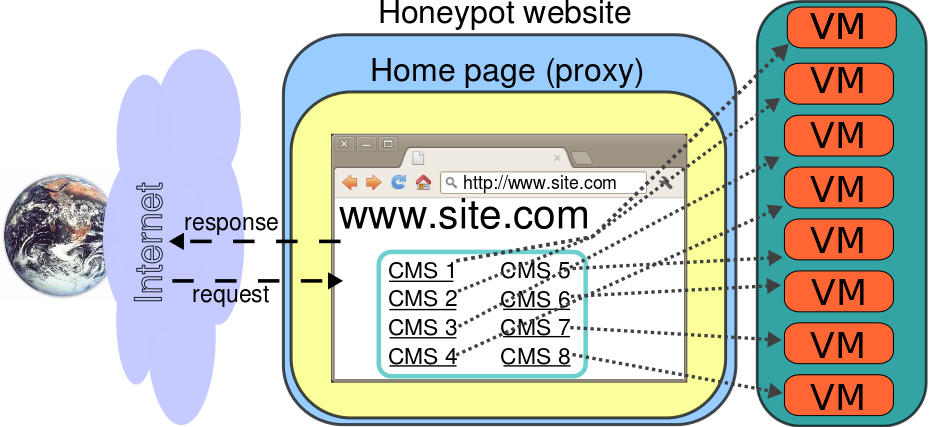
\includegraphics[width=0.9\textwidth]{Images/websiteOverview.png}}
\caption{Overview of a website.\label{fig:websiteView}}
\end{figure}

As can be seen, the system is composed by two main parts: A VMWare server, located in our facilities, hosting our web applications, and a total of 500 replicated web proxies hosted by TrendMicro distributed over eight different locations across the world, connecting the servers to the Internet. Any request reaching one of the web proxies is forwarded to our server, and the suitable response is sent back to the proxy and from there to the final user.

To make our honeypots reachable from web users, we purchased 100 bulk domain names on GoDaddy.com with privacy protection. The domains were equally distributed among the .com, .org, and .net TLDs, and assigned evenly among the locations.
On each of the eight locations, we configured four additional subdomains for every domain, obtaining five distinct websites (e.g, on domain site.com we have www.site.com, sub1.site.com, sub2.site.com, sub3.site.com and sub4.site.com). A schema of this structure is shown in Figure~\ref{fig:genSchema}. The total number of websites obtained in this way is 4000.

\begin{figure}[tbh]
\centerline{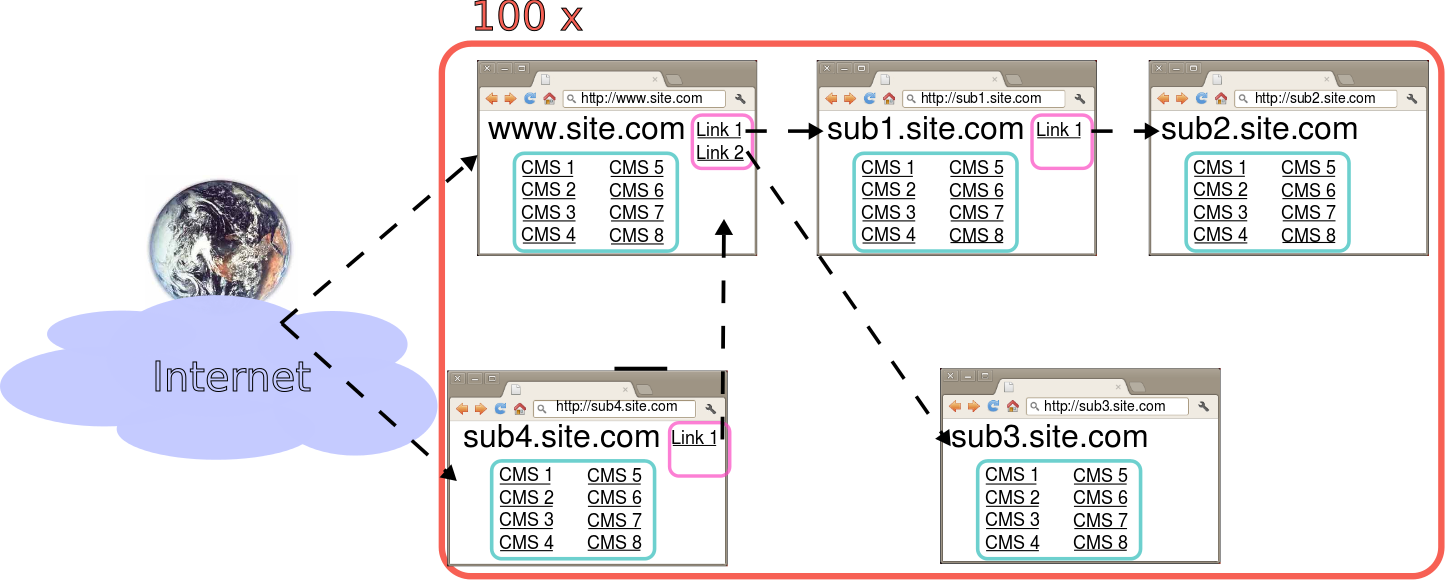
\includegraphics[width=0.9\textwidth]{Images/GeneralSchema.png}}
\caption{General schema of the honeypot platform.\label{fig:genSchema}}
\end{figure}

Finally, we advertised the 500 domains on the home page of the authors and on the research group's website by means of transparent links. This approach, initially proposed by M\"uter et al. \cite{hihat}, consist in adding on high-reputation web pages links not visible by the user to other pages, so that the position of these latter ones in the Google index will increase.

In order to manage such a high-number of different machines in a comfortable way we used a modified version of \emph{ftp-deploy} script to upload, in batch, every file we needed to each of the 500 websites in our possession. This greatly simplified the deployment and the update/upgrade of the system, and solved one of the main issues developers need to solve during the deployment of replicated content over different providers. Even if the hosting services can always be traced back to Trend MicroSystems, in fact, each of them has its own directory structure and specific web interface, discouraging the usage of ssh and other advanced management options in order to deploy contents. Thus the only way to easily perform this action is to use FTP protocol, the only one supported by every provider.

Looking more closer to figure~\ref{fig:genSchema}, It can be noticed as the linking structure is not the same for every subdomain. Indeed, each subdomain links to at most 2 different subdomains under its same domain. The aim of this particular structure of the linking graph is to detect possible malicious traffic from systems that automatically follow links and perform automated attacks or scans.

\section{The Web Applications}
We deployed a total of eight web servers, using seven web applications and one static website linked to 17 pre-installed web shells. Every web application is based on an open source Content Management System among the most used across the Internet, each one based on php version 5 and using (if needed) MySQL version 5 as RDBMS. For each CMS, we chose a version with a high number of reported vulnerabilities, or at least with a critical one that would allow the attacker to take full control of the application. We also limited our choice to versions no more than 5 years old in order to ensure our websites are still of interest to attackers.
Our choice was guided by the belief that attackers are always looking for low-hanging fruits. On the other hand, our honeypots will probably miss sophisticated and unconventional attacks, mostly targeted to high profile organizations or well known websites. However, these attacks are not easy to study with simple honeypot infrastructures and are therefore outside the scope of our study.

\begin{description}
\item[phpMyAdmin: ] phpMyAdmin \cite{phpMyAdmin} is an open source tool written in PHP for the administration of a MySQL database over the WWW. The version installed is the 3.0.1.1 disguised as version 2.6.4-rc1. Both these versions present a critical PHP code injection vulnerability in the ``/scripts/setup.php'', a page needed during the installation process of the CMS which should be manually deleted at the end of it, allowing an attacker to inject a payload that can execute arbitrary PHP commands. Even if both versions are vulnerable to this exploit, a research over various underground forums shows as the one for the version 2.6.4-rc1 is far more well-known with respect to the 3.0.1.1 one (even if they are identical), thus we disguised our version to the one more suitable for attackers (the 2.6.4-rc1 version of this CMS is no more available for download on phpMyAdmin website).
Reference:
\begin{itemize}
\item
\url{http://www.exploit-db.com/exploits/8921/}
\end{itemize}

\item[osCommerce: ] osCommerce \cite{osCommerce} is one of the most used openSource e-commerce and online store-management frameworks. Our specific version is the 2.2, which contains several critical vulnerabilities, from arbitrary file upload to modification of admin user and password by anonymous user.
Reference:
\begin{itemize}
\item
\url{http://www.exploit-db.com/exploits/16899/}
\item
\url{http://www.exploit-db.com/exploits/9566/}
\item
\url{http://www.exploit-db.com/exploits/10707/}
\item
\url{http://www.exploit-db.com/exploits/12801/}
\end{itemize}

\item[Joomla!: ] Joomla! \cite{joomla} is an open source general-purpose framework. The version we used is the 1.5, with the addition of two plugins, tinybrowser 1.0 (a plugin for listing directories and file management) and com\_graphics 1.0.16 (magnify ability to the page). This web application suffers from several vulnerabilities both on server and on client side, like admin password reset, remote file inclusion, local file inclusion and multiple XSS (Cross-Site scripting) caused by bad input filtering.
Reference:
\begin{itemize}
\item
\url{http://www.exploit-db.com/exploits/6234/}
\item
\url{http://www.exploit-db.com/exploits/16091/}
\item
\url{http://www.exploit-db.com/exploits/12430/}
\item
\url{http://www.exploit-db.com/exploits/9926/}
\end{itemize}

\item[Wordpress: ] Wordpress \cite{wordpress} is a popular CMS aimed to the easy creation of a blog. Our version is the 2.8, with one plugin installed, kino version 1.1, a calendar/event manager, and a theme, amphion-lite. Both the plugin and the theme rely on the file timthumb.php, vulnerable from Remote File Inclusion vulnerability. This is a website which allowed to post comments, therefore we needed to take care of removing offensive/illegal content from the posts. Anyone can register to the website, and the default user role is Contributor, allowing creation of posts with links but not file uploads. Posts are sanitized from links and then become viewable to guests. For this particular machine we had to authorize sending emails because of the registration procedure, but we stop email scams by the analysis of the content of each single mail the server is willing to send.

Reference:
\begin{itemize}
\item
\url{http://www.exploit-db.com/exploits/17872/}
\end{itemize}

\item[SMF: ] SMF (acronym of Simple Machines Forum \cite{smf}) is an open source software for developing a forum web application, where users can open threads and post comments. Our specific version is the 1.1.3. As in the case of Wordpress, we applied the same approach for managing registration via mail and for checking posts on the forum. This application suffers from several vulnerabilities, the most important ones are a remote PHP remote code execution vulnerability and an information-disclosure vulnerability.
Reference:
\begin{itemize}
\item
\url{http://www.exploit-db.com/exploits/10274/}
\end{itemize}

\item[Static website: ] We also created a static website composed only by HTML pages with a hidden directory containing 17 different web shells. These web shells have been taken from underground forums and past experiments, and are fully equipped in order to perform any operation an attacker would like to perform, from shell commands execution to full database dump. They are indexable by search engines and can therefore easily be found by an appropriate dork.

\item[Wordpress: ] Because of the dominant position of Wordpress on the market, we deployed another web application based on this CMS. This specific machine run an updated version of Wordpress (3.4) with two plugins, wpstorecart and nextgengallery. Both these plugins suffer from Arbitrary File Upload vulnerability.

\begin{itemize}
\item
\url{http://www.exploit-db.com/exploits/19023/}
\item
\url{http://1337day.com/exploit/description/20352}
\end{itemize}

\item[Drupal: ] Drupal \cite{drupal} is the third most common CMS present on the web, after Wordpress and Joomla!. We installed version 7 of this application with IMCE plugin (Image manager). This machine does not present a standard vulnerability, but rather a mis-configuration: IMCE allows for remotely upload files inside a specific directory, and its access should be denied for every user but the administrator. In this case this page is usable by every user, and it's also indexable by search engines.
\end{description}

Table~\ref{tab:webapps} shows a summary of the web applications used and its vulnerabilities.

\begin{table}[tbh] % per piazzare la tabella t:top b:bottom h:here in ordine di preferenza; h è sconsigliato
\begin{center}
\begin{tabularx}{\textwidth}{|c|X|X|X|X|}
\hline
\textit{VM \#} & \textit{CMS, version} & \textit{Plugins} & \textit{Description} & \textit{Vulnerabilities} \\
\hline
1 & phpMyAdmin, 3.0.1.1 & - & MySQL database manager & PHP code injection \\
2 & osCommerce, 2.2 & - & Online shop & 2 remote file upload, arbitrary admin password modification \\
3 & Joomla, 1.5.0 & com\_graphics, tinymce & Generic / multipurpose portal & XSS, arbitrary admin password modification, remote file upload, local file inclusion \\
4 & Wordpress, 2.8 & kino, amphion lite theme & Blog (non moderated comments) & Remote file include, admin password reset \\
5 & Simple Machines Forum (SMF), 1.1.3 & - & Forum (non moderated posts) & HTML injection in posts, stored XSS, blind SQL injection, local file inclusion \\
6 & PHP web shells, static site & - & Static site and 17 PHP shells (reachable through hidden links) & PHP shells allow to run any kind of commands on the host \\
7 & Wordpress, 3.4 & wpstorecart, nextgengallery & Blog & Arbitrary File Upload \\
8 & Drupal, 7.0 & IMCE & Generic / multipurpose portal & Remote File Upload \\
\hline
\end{tabularx}
\caption{Summary of the web applications deployed on the system.\label{tab:webapps}}
\end{center}
\end{table}

\section{The Web Proxy}

The Web Proxy is in charge of receiving requests from the Internet, creating a unique channel for the communication between the user and the vulnerable web server and propagating them to the gateway.
All web applications are hosted in our facilities, in eight isolated virtual machines running on a VMWare server. On the proxy hosting side we installed only an ad-hoc proxy tool (HoneyProxy) in charge of forwarding all received traffic to the right virtual machine on our server.

We crafted a custom installation of the Apache web server using modified .htaccess file, ModRewrite module, cURL module and php.ini configuration files, in order to be able to transparently forward user requests to the appropriate URL on the corresponding virtual machine. Any attempt to read a non-existing resource, or to access the proxy page itself would result in a usual 404 error page shown to the user. Not taking into account possible timing attacks or intrusions on the proxy, there is no way for a visitor to understand that he is speaking to a proxy.

The HoneyProxy system installed on every website is composed of an index file, the PHP proxy script itself and a configuration file. The index file is the home page of the website, and it links to the vulnerable web applications and to other honeypot websites, based on the contents of the configuration file. The proxy uses sessions in order to serve the appropriate page to each user, and it also scans each response received from the web application before forwarding it in order to substitute each domain with the one initially requested by the user.

Furthermore, The PHP proxy adds two custom headers to each request it receives from a visitor:

\begin{description}
\item[X-Forwarded-For: ] this standard header, which is used in general by proxies, is set to the real IP address of the client. In case the client arrives with this header already set, the final X-Forwarded-For will list all the previous IPs seen, keeping thus track of all the proxies traversed by the client. This is necessary in case the user passes through another proxy before reaching ours.

\item[X-Server-Path: ] this custom header is set by our PHP proxy in order to make it possible, for us, to understand the domain of provenance of the request when analyzing the request logs on the virtual machines. An example of such an entry is: X-Server-Path: http://sub1.site.com/. This entry will be used to substitute all references to other resources inside each page before sending it to the user.
\end{description}

These two headers are transmitted only between the hosting web server and the honeypot VM's web server, and thus they are not visible to the users of the HoneyProxy.

\section {The Gateway}

The Gateway is in charge of sorting requests coming from the proxy to the appropriate web server. This is the only communication channel between the vulnerable web applications and the outside world, and it's therefore a critical point for the infrastructure.
This machine runs a very basic Debian version, with a complex routing table and a complete set of firewall rules based on iptables. We provided this machine with two connections to the Internet: the main one, where the requests to/from the honeypots are going through, which is based on a point-to-point VPN connection to the proxy, and a secondary line which is directly connected to the outside world via a DSL connection.

The general approach on which the gateway relies in order to solve connections is the following:

\begin{description}
\item[Requests coming from the proxy: ] these requests are coming from the point-to-point VPN connection. The proxy already changed the request in such a way that the destination port will be specific to the web application the request is directed to. The proxy simply receives the request, changes the destination port to the usual 80 and sends the request to the appropriate web application.

\item[Request coming from a web application: ] when the gateway receives a request coming from one of the web servers, it tries to understand its nature. If it's an HTTP response, it will forward it to the Proxy as a normal gateway, if it's something else (a beginning SSH connection, a raw IP packet or something else) it will immediately drop the request and dump it on a log which will be analysed daily. There are two exceptions to this behaviour, explained in the following points.

\item[DNS requests coming from a web application: ] DNS requests represent an exception to the normal behaviour. This kind of requests are forwarded to the Internet by the gateway using the secondary line. This behaviour allows for the request to be solved without passing through the web proxy. The proxy, in fact, is not hosted in our facilities and some malicious DNS could be blocked by the hosting provider. In this way we are sure that every DNS request is solved independently from the target of the request.

\item[HTTP requests coming from a web application: ] this represents the second class of exceptions to the normal behaviour of the gateway. In this case, in fact, we want to log the content of the HTTP request, which would be impossible if we instantaneously drop the first packet received. The natural sequence of actions performed during such an event is, in fact:
\begin{itemize}
\item an initial TCP SYN packet from the client to the server;
\item the server will answer with a TCP SYN/ACK packet;
\item the client will send a TCP ACK packet and the actual HTTP request;
\end{itemize}
Because we are interested in the last one of these packets, we used an extension of iptables called ``conntrack'' \cite{conntrack}, allowing for tracking the entire connection. Using this extension we manage to stop (and log) the connection when the first HTTP request is performed.
\end{description}

\section{The VMWare Server}
\label{sec:vwmwareserver}

The VMWare server is the container of our web applications. Each web application is encapsulated in a different virtual machine hosted on this server. This allows for a fast recovery of any web application after a successful attack; this recovery is performed daily.
Our aim is to provide a properly safe environment for each web application, guaranteeing not only the undetectability of the presence of the virtual machine (the attacker should think to face a normal web server, not a honeypot), but also disallowing any action that can harm any other system outside our honeypots (e.g., in case a DoS script toward another server is run from one of our machines). Furthermore, we needed to prevent our honeypots to host any malicious or illegal content that could be dangerous for any legitimate client visiting the webpage.
We studied every possible threat that could endanger our honeypot system, and we tackle each of these problems separately.

\subsubsection{Gaining high privileges on the machine}

 We tackled this problem by using a double protection. First, all our web application run in a completely updated VMWare virtual machine, which is considered pretty safe (the last known escaping vulnerability is CVE-2008-0923 by Core Security Technologies \cite{vmescape}). On this virtual machine there is a further protection, as the vulnerable processes run inside an LXC container. This technology provides an operating system-level virtualization that has its own process and network space. Basically we are building multiple cages one inside the other in order to guarantee that no possible attacks can reach our real machine. Inside this container, we installed only basic linux tools (in particular, they are python, perl, wget, cURL, build-essentials) and the two services needed for the web application to work, Apache and mysql. This approach does not guarantee absolute protection, but in order to reach the real servers an attacker should need at least one 0-day exploit for Apache, one for LXC and one for VMWare, which is obviously a very remote possibility.

\subsubsection{Using the honeypot machine as a stepping stone to launch attacks or email campaigns}

 This is probably the most important threat a high-interaction honeypot system should face when it's been deployed on the Internet. We wanted to trick the attacker into feeling that his attack worked, but without actually doing any real action instructed by the malicious user. Outgoing connections starting from our machine are blocked by a specific set of \emph{iptables} rules. Furthermore, the connMark plugin for iptables allowed us to fool the attacker into thinking the machine can actually connect to the outside. As mentioned before, we allow the first and second packet in the TCP three-way handshake , but we disallow the final third packet. This provokes most of the tools used to establish a TCP connection (wget, cURL, netCat) to display a \emph{``Connection Established''} message, tricking the attacker into thinking that the outside server is suffering from connectivity problems. Furthermore, this allowed us to collect not only data relative to the IP of the target server, but also specific queries, as specific web addresses of malicious scripts. We also set a limit to the maximum number of connections that can be established in this way between one of our servers and an outside world in order to prevent our servers to be used as a SYN flood Denial Of Service attack starting platform.

\subsubsection{Hosting and distributing illegal content(e.g., phishing pages)}

 It is virtually impossible to completely disable this threat if our web applications have remote file upload vulnerability. An attacker could always upload a phishing pack and then advertise the link to it using another server, fooling the victims into visiting the malicious page and inserting their credentials. In any case, we mitigate this risk by limiting the directories where files can be uploaded and preventing any modification to existing files on the machine, so that attackers can't, for example, replace the index page of our web servers. As a precautionary measure, we also monitor every change happened in the LXC container file system and in the VM. If such a modification is detected, the system takes a snapshot of the VM. Each VM is restored to its original snapshot at regular intervals, preventing potentially harmful content from being delivered to victims or indexed by search engines.

\subsubsection{Illegal promotion of goods or services (e.g., spam links)}

 Some of our applications allowed for some degree of interaction with users from the Internet, like insert comments to blog entries or publish posts in case of the forum. This kind of applications are heavily targeted by spammers, and we wanted to be sure that links and posts published by malicious users would not reach regular users or be indexed by search engines. Luckily for us this activity is almost fully accomplished by automatic scripts, therefore we were able to directly modify the source code of the interested web application, commenting out each snippet of code responsible of showing any spam link or related content. In this way, attackers can still publish content (and we log every single post they make), but a manual check of the webpage would show a blank message instead of the malicious' payload.


\chapter{Data collection, analysis and visualization}

\section{Introduction}

We developed a specific set of software in charge of the collection and analysis of data received from the honeypot system.
We basically have two kinds of data collected:
\begin{description}
\item[Requests: ] Once the attacker exploits a vulnerability on a honeypot, he will probably try to download files from other servers on the Internet or perform other types of requests to some external sources. We collect most of these data through the gateway. The only exception is represented by HTTPS connections: this kind of connection won't show up on the log at the gateway level, as the SSL handshake can't be completed (the connection is dropped before). We inserted a backdoor inside the OpenSSL library, precisely inside the SSL\_write function, in order to log in clear text the content of the request.

\item[Files: ] We deployed most of the vulnerable web servers with an Arbitrary Upload File vulnerability, because we are interested in collecting files attackers use during their hacking activity. Other than original files uploaded, we also want to detect if the same file is used by different attackers, and track any modification happened on the file while being used from different people.
\end{description}

The whole software is completely written in Python, using a MySQL database to store informations.

\section{Acquisition}

The acquisition of data is a pivotal part of the architecture: as mentioned before, requests are collected via live-logging using the log chain of iptables, while HTTPS requests are directly logged by our backdoor; regarding uploaded files, we use two different systems of acquisition:

\begin{description}
\item[Original files] are collected by a direct analysis of the requests: because of the fact we know the vulnerability, we can easily scan all HTTP requests looking for specific patterns that are used during the exploitation phase: by looking at the content of these requests, we can build the original content of the uploaded file;
\item[Modified files] are collected at constant interval: every five minutes our system takes a snapshot of the files present on the web server, compares this snapshot with the ``basic'' one (the snapshot that will be used for the reboot of the machine every day), takes all files that are not present in the latter one and compares them to the one saved before during the same day: if any new file show up, or if an old file has been modified, the new version of the file is saved.
\end{description}

This system allows us to collect every file uploaded and most of the modifications happened on them during the day.
Other than saving these files in a specific folder related to the day of acquisition and the web application they were uploaded to, we also save their MD5 inside a specific database. In case that file is already present in our system, it will be immediately deleted, in order to optimize storage space.

\section{Analysis}

We perform different analysis both over the uploaded files and the requests, like deobfuscation, categorization and cross-checking with other databases.

\subsection{Analysis of Requests}
\label{sec:SectionReqAnalysis}
Even if we collect and store in a database all kinds of requests we receive, we decided to analyse in more details only HTTP/HTTPS requests for the moment, further analysis will may be performed in the future.
First of all, we collect the complete URLs from the HTTP/HTTPS requests, and we integrate these data with a list of URLs we extract directly from the uploaded files. We filter this list from a range of blacklisted domains, like youtube, facebook and image hosting websites. We send this list of URLs to another machine, which will perform a GET request for all these URLs by using a DSL connection. In this way, even if the web server we are connecting to is owned by an attacker who is checking his logs, there is no possibility for him to discover our presence. All files collected in this way are added to the group of files collected during the day, ready for being analysed.

\subsection{Analysis of Files}

Our aim is to categorize files according to their similarity, in order to identify not only its general category (Web Shell, bruteforce script etc) but also it's subtype/family. This objective can be accomplished only by examining every single file and making it suitable for a clusterization.
The analysis is performed through various steps, each of them will be explained in details.

\subsubsection{Type Categorization}
This categorization is related to the intrinsic type of the file, like PHP script, HTML document etc.
We used the libMagic \cite{libmagic} library, the same used by the \emph{file} Unix command to identify the file type of an entity, with a particular improvement: many attackers, in fact, disguise their files by tampering the signature responsible for the recognition of the type, adding on top of the normal one another one for making them appear as images, in order to trick basic automatic file type checkers present on CMSs. In order to comply with this behaviour, we determine the type of a certain file once, and if it's categorized as Image, we repeat the same operation by removing the first 16 bytes of the element. In this way, if any other signature has been added, we can retrieve the correct file type, and in the opposite case we are simply getting as output ``data''.

If the file is categorized as Image, Audio or Video it is immediately removed by the system in order to save storage space.

\subsubsection{Deobfuscation}
Deobfuscation of PHP scripts is a fundamental part of the analysis process: more than 70\% of the PHP scripts we receive are in fact obfuscated in several ways, from a simple hex encoding in order to fool eventual Web Application Firewall up to complex obfuscating systems provided by specific software, like php-crypt \cite{phpcrypt}.
For very easy obfuscation systems, like hex-encoding or url-encoding of ASCII characters, we can easily obtain the deobfuscated version by using the decode feature of the string library present in Python.
However, most of the obfuscation scripts work by performing several operations on a string and then evaluating it in order to run some code. We created \emph{Transformer}, a software aimed for the secure deobfuscation of PHP files to handle this situation.

In PHP (up to version 5), we basically have two different ways for evaluating a script:
\begin{itemize}
\item \emph{eval} command, which takes a string as input, and does a direct evaluation of the string (example: \code{eval(\'echo \"Hello World\";\');});
\item \emph{preg\_replace} command, when used with ``e'' inside the pattern input as PREG modifier. In this case, the command looks for a certain pattern, replaces it with the replacement input, and then automatically evaluates the resulting output\\(example: \code{preg_replace(\"/.*/e\",\'print(\"Hello World\")\',\"\");}) %forced return because code does not follow usual margins
\end{itemize}

In order to bypass WAFs (Web Application Firewalls) and IDS (Intrusion Detection Systems), which are signature-based software, attackers tend to obfuscate their code, which will be deobfuscated and evaluated at runtime using one of these two functions.
We also noticed, during our analyses, that is not uncommon to find, inside PHP files, a small base64-encoded string, which is evaluated at runtime. The code, deobfuscated, reveals in most of the cases to be a \emph{sendmail} function directed to the creator of the file (who is often different from the person who is actually using it), in order to notify him about a new target uploaded.

There are several ways for deobfuscating a PHP file, from a web service \cite{webdeobf} to the \emph{EvalHook} PHP extension developed by Stefan Esser \cite{evalhook}. All of them revealed some problems for being used in our case:
\begin{itemize}
\item we need to deobfuscate a huge amount of files per day, and a web service can't cope with this requirement;
\item evalhook library works by actually executing the non-deobfuscated code, an action we want to avoid in order not to cause any harm to our system.
\end{itemize}

Our software, \emph{Transformer}, is able to hook eval-related calls found inside the source-code, go backward from the position of the call looking for possible transformations of the input parameters, create a new PHP file containing the strictly necessary for the deobfuscation and finally deobfuscate the code, replacing the call with the deobfuscated result inside the original file. This operation is performed recursively, in order to cope with several layers of obfuscation, everything without any need for user interaction.
It must be noticed that we are not performing a global parsing of a PHP file, because the language itself cause this operation to be really challenging and time/performance consuming.

By using this approach we reached fairly high success rates (on our experiments, more than 80\%), with the advantage of being reasonably safe from executing harmful code. We enforce our security by running this code in a virtual environment, which is restored on a daily basis.

\subsubsection{Normalization}
Our aim is to clusterize files based on their similarity, and one of the most important operations for improving our classification system is to perform a normalization of them.
Because of the different nature of the files received, from source code to HTML pages and executables, we developed several rules for removing ``user-specific'' parts according to the type of file currently analysed.
For example, when dealing with PHP source code files we are using the following set of rules:
\begin{itemize}
\item removal of extra whitespaces, normalizing every line for having single whitespaces and single new-line character (``\bs n'');
\item removal of empty PHP tags resulting from deobfuscation (sequences of \code{<?php ?>} or \code{<? ?>}); %TODO: correct!!
\item removal of C-style comments, both in single line version (using \code{//}) and multi-line (\code{/*...*/});
\end{itemize}

Because most of these files are dealing with HTML tags, we also remove any sign of user-specific tags or graphical tags inside the code, removing \code{<style>} contents, \code{<meta>} ones and HTML comments.

Last, we remove any sign of user-specific content, as phone numbers, e-mails and URLs present inside the file. The URLs will be saved for further analysis (cfr. Section ~\ref{sec:SectionReqAnalysis}).

\subsection{Clustering}
What we obtain from \emph{Transformer} output is a normalized and anonymized file, which is ready to be clustered by our system. We use three different systems for clustering files: sdhash, ssdeep, md5.

\subsubsection{Sdhash}
Sdhash is our first resource for computing similarity between files. Based on the working of Vassil Roussev \cite{sdhash}, this tool produces a digest for each file. In details, it tries to find from every file the features (64-byte sequences) that have the lowest empirical probability of being encountered by chance. Each of the selected features is hashed and placed into a Bloom filter (a probabilistic set representation). When a filter reaches its capacity, a new filter is created until all the features are accommodated. Thus, a similarity digest consists of a sequence of Bloom filters and its length is about 2-3\% of the length of the input. Bloom filters have predictable probabilistic properties, which allow for two filter to be directly compared using a Hamming distance-based measure. The result gives an estimate of the fraction of features that two filters have in common that are not due to random chance.
To compare two digests, for each of the filters in the first digest, the maximum match among the filters of the second is found. The resulting matches are then averaged.

This technique has been proved as extremely successful for text-based files, and based on the results from Roussev (ref~\ref{fig:sdhash_tp_fp}) we chose a threshold value of 70 for considering two files as similar.

\begin{figure}[tbh]
\centerline{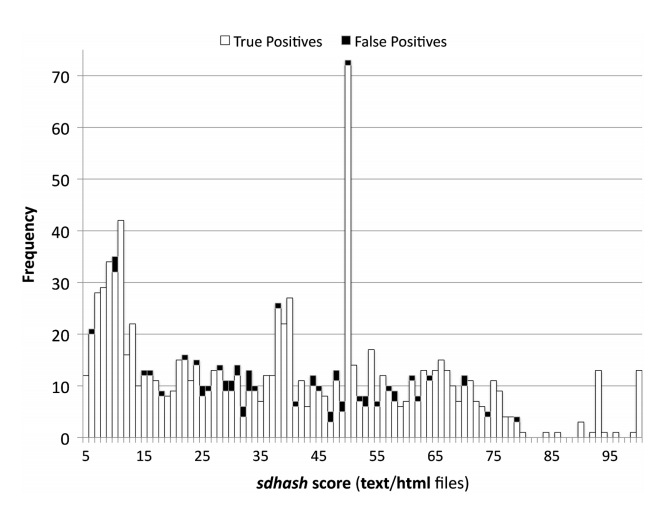
\includegraphics[scale=1]{Images/sdhash_TP_FP.jpg}}
\caption{Results of sdhash similarity score with HTML files.\label{fig:sdhash_tp_fp}}
\end{figure}

The only disadvantages of sdhash computation are the fact that the resulting hash size is directly proportional to the size of the file, which can be a problem when storing the hash (as we do), and the minimum file size requested for sdhash to work, which is 4096 B, a value that can't be satisfied when dealing with small configuration files uploaded (e.g., a .htaccess file).

\subsubsection{Ssdeep}
Ssdeep is one of the best-known techniques for detecting similar files. It's been invented by Jesse Kornblum \cite{ssdeep} in 2006 and based on the work on spam detection performed by Andrew Tridgell \cite{spamsum}.
The system is based on the concept of piecewise hashing. A piecewise hashing uses an arbitrary hashing algorithm (in Ssdeep case is FNV) to create many checksums for a file instead than just one. Rather than generating a single hash for the entire file, a hash is generated for many discrete fixed-size segments of the file. Once we obtained all these pieces, Ssdeep uses a rolling hash algorithm for creating a Context Triggered Piecewise Hash (CTPH). Such hashes can be compared in order to identify ordered homologous sequences between files.

This approach produces worse results than Sdhash (ref~\ref{fig:sdhash_ssdeep}), but it has the advantage of obtaining a fixed-size hash (which is easier to store in a database) and it accepts files having a smaller size, 2048 B.

\begin{figure}[tbh]
\centerline{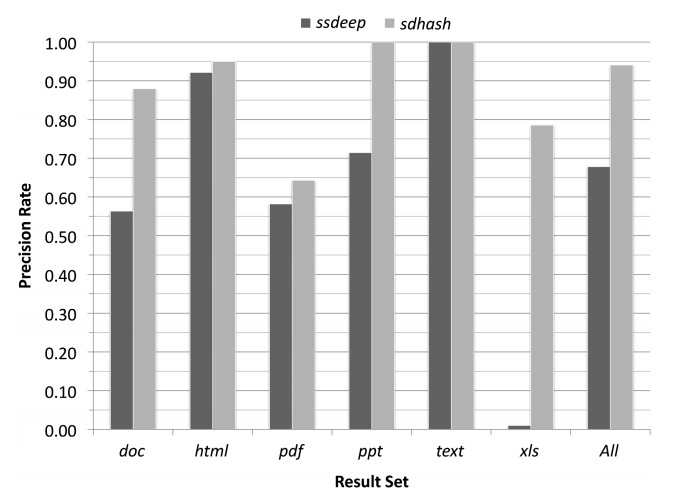
\includegraphics[scale=0.9]{Images/sdhash_ssdeep.jpg}}
\caption{Comparison of the precision rate of Ssdeep and Sdhash over different file types\label{fig:sdhash_ssdeep}}
\end{figure}

\subsubsection{MD5}
MD5 is a well-known technique for creating cryptographic hash of files. Designed by Ron Rivest and published by IETF as RFC 1321 \cite{md5}, this technique is based on different non-linear functions computed on fixed size input in order to achieve a 128 bit hash value.

This is the last technique we use for computing similarities: whenever the file is too short to apply Sdhash or Ssdeep, we use this algorithm in order to find if the normalized output of the file is the same of another file, showing its similarity.


\chapter{Results}

\section{Overview}

The experiments run for a period of 100 days, from the August 1st 2013 to November 9th, 2013. During this period, we collected 9.5 GB of raw HTTP requests, consisting in approximately 11.0M GET and 1.9M POST. Our honeypots were visited by more than 73,000 different IP addresses, spanning 178 countries and presenting themselves with more than 11,000 distinct User-Agents. This is over one order of magnitude larger than what has been observed in the previous study by John et al. on low interaction web-application honeypots \cite{johnhsh}. Moreover, we also extracted over 110,000 files that were uploaded or modified during attacks against our web sites, 85,000 of them are unique.
There are two different ways to look at the data we collected: one is to identify and study the attacks looking at the web server logs, and the other one is to try to associate a goal to each of them by analyzing the uploaded and modified files. In the first part of this chapter we will look at the first part, while in the second we will give some examples of uploaded files, in order to understand attacker's goals.

\textcolor{blue}{NOTE: maybe remove Overview, as it's closed in itself (we are starting with another section for obtaining nice subsections based on the different phases)}

\section{Exploitation and Post-Exploitation Behaviors}

While analyzing the behavior of attackers lured by our honeypots, we identified four different phases commonly present in an attack session: discovery, reconnaissance, exploitation, and post-exploitation. The \emph{Discovery} phase describes how attackers find their targets, e.g. by querying a search engine (using a dork) or by simply scanning IP addresses. The \emph{Reconnaissance} phase contains information related to the way in which the pages were visited, for instance by using automated crawlers or by manual access, and if this manual access is performed via visual browser or command line tool, and if the attacker is using an anonymization proxy. In the \emph{Exploitation} phase we describe the number and types of actual attacks performed against our web applications. Some of the attacks reach their final goal themselves (for instance by changing a page to redirect to a malicious website), while others are only uploading a second stage. In this case, the uploaded file is often a web shell that is later used by the attacker to manually log in to the compromised system and continue the attack. We refer to this later stage as the \emph{Post-Exploitation} phase.

It must be noticed, however, that not all phases are present in every attack: some of them can be joined in one step (e.g., reconnaissance and exploitation are often performed in one single action), some of them are simply not present (e.g, post-exploitation), some visits do not lead to an actual attack (error in attackers requests, or incomplete file upload), and sometimes it is just impossible to link together different actions performed by the same attacker with different IP addresses.

Neverthless, by extracting the most common patterns from the data collected at each stage, we can identify the ``typical attack profile'' observed during our experiments with the following sequence:

\begin{enumerate}
\item
69.8\% of the attacks start with a scout bot visiting the page. The scout often tries to hide its User Agent (removing directly the header) or disguise themselves as a crawler search (the most used being \emph{GoogleBot});
\item
Few seconds after the scout has identified the page as an interesting target, a second automated system (hereinafter exploitation bot) visits the page and executes the real exploit. This is often a separate script that does not fake the user agent, therefore often appearing with strings such as \emph{libwww/perl}.
\item
If the vulnerability allows the attacker to upload a file, in 46\% of the cases the exploitation bot uploads a web shell. Moreover, the majority of the attacks upload the same file multiple times (in average 9, and sometimes up to 40), probably to be sure that the attack was successful.
\item
After an average of 3 hours and 26 minutes, the attacker logs into the machine using the previously uploaded shell. The average login time for an attacker interactive session is 5 minutes and 37 seconds.
\end{enumerate}

While this represents the most common behavior extracted from our dataset, many other combinations were observed as well - some of which are described in the rest of the section. Finally, it is important to mention that the attack behavior may change depending on the application and on the vulnerability that is exploited. Therefore, we should say that the previous description summarizes the most common behavior of attacks against osCommerce 2.2 (the web application that received by far the largest number of attacks among our honeypots). A particular notice must be performed regarding the SMF application: this application suffered from heavy traffic, provoked by automated bots, and we preferred to exclude this application from our statistics in order to produce more reliable results. A specific discussion over the content of messages posted on the forum will be performed later. In Figure ~\ref{fig:overview_phases} we show an overview of the four phases and its characteristics.

\begin{figure}[tbh]
\centerline{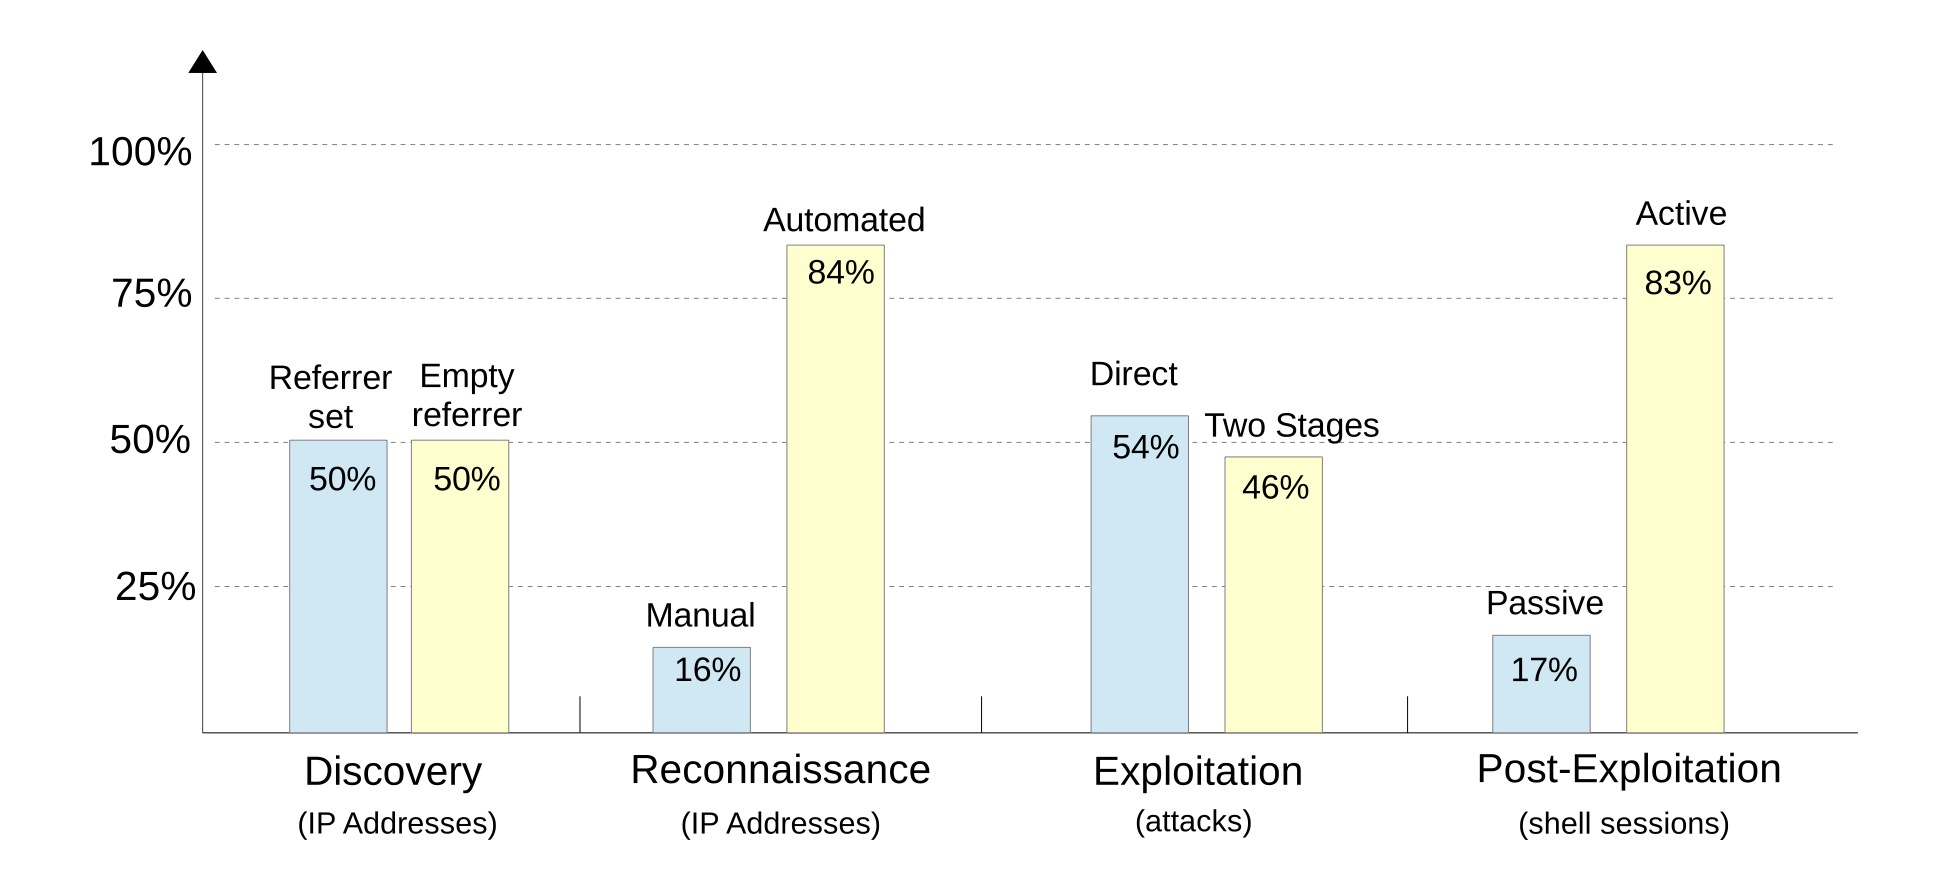
\includegraphics[scale=0.4]{Images/overview_phases.jpg}}
\caption{Overview of the four phases of an attack\label{fig:overview_phases}}
\end{figure}

\subsection{Discovery}
The very first HTTP request hit our HoneyProxy only 10 minutes after the deployment, from ``Googlebot''. The first request not related to a benign crawler came after 1 hour and 50 minutes.
During the first few days, most of the traffic was caused by benign web crawlers. Therefore, we designed a simple solution to filter out benign crawler-generated traffic from the remaining traffic. Since HTTP headers alone are not trustable (e.g., attackers often use User Agents such as ``Googlebot'' in their scripts) we collected public information available on bots and we combined them with information extracted from our logs and validated with WHOIS results in order to identify crawlers from known companies. By combining User Agent strings and the IP address ranges associated to known companies, we were able to identify with certainty 14 different crawlers, originating from 1965 different IPs. Even though this is not a complete list, it was able to successfully filter out most of the traffic generated by benign crawlers.

\begin{figure}[tbh]
\centerline{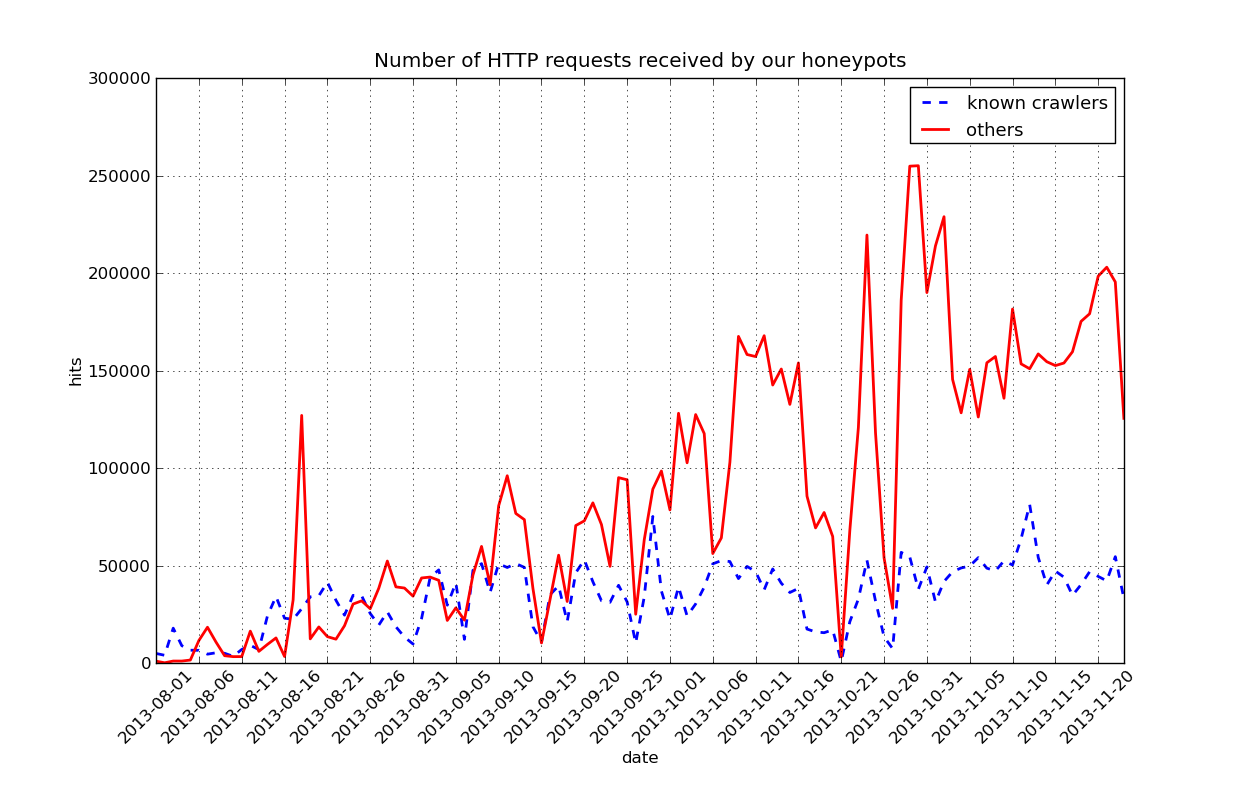
\includegraphics[scale=0.4]{Images/requestsCrawlers.png}}
\caption{Overview of the four phases of an attack\label{fig:requestsCrawlers}}
\end{figure}

Some statistics about the origin of the requests is shown in Figure ~\ref{fig:requestsCrawlers}. The amount of legitimate crawler requests is more or less stable in time, while, as time goes by and the honeypot websites get indexed by search engines and linked on hacking forums or on link farming networks, the number of requests by malicious bots or non-crawlers has an almost linear increase.
While looking at these statistics we also noticed a number of suspicious spikes in the number of accesses. In several cases, one of our web applications was visited, in few hours, by several thousands of unique IP addresses (compared with an average of 192 per day), a clear indication that a botnet was used to scan our sites.

Interestingly, we observed the first suspicious activity only 2 hours and 10 minutes after the deployment of our system, when our forum web application started receiving few automated registrations. However, the first posts on the forum appeared only four days later, on December 27th. Even more surprising was the fact that the first visit from a non-crawler coincided with the first attack: 4 hours 30 minutes after the deployment of the honeypots, a browser with Polish locale visited our osCommerce web application and exploited a file upload vulnerability to upload a malicious PHP script to the honeypot. We also examined the IP source address in order to understand the more active countries, as we can see from ~\ref{fig:requests_countries} China, Russia, and USA are in order the top three countries for number of requests. \textcolor{blue}{HEATMAP OR PIE CHART?}.

\begin{figure}[tbh]
\centerline{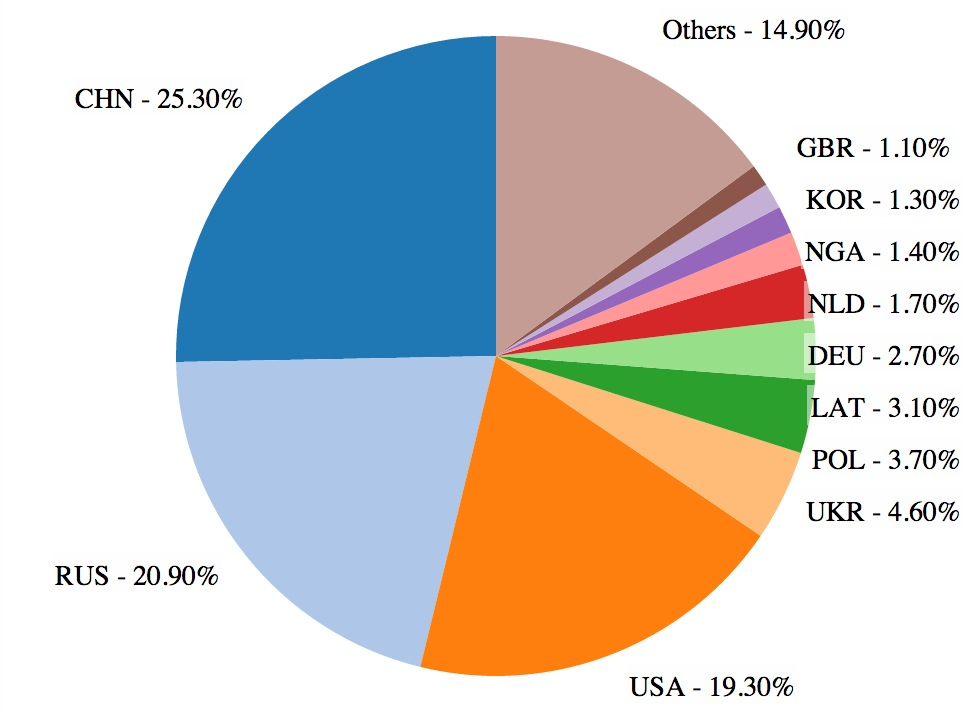
\includegraphics[scale=0.5]{Images/requests_countries.jpg}}
\caption{Number of requests divided by country\label{fig:requests_countries}}
\end{figure}

\subsubsection{Referer Analysis}

The analysis of the Referer HTTP header (whenever available) helped us identify how visitors were able to find our honeypots on the web. Based on the results, we can distinguish two main categories of users: attackers using search engines to find vulnerable applications, and victims of phishing attacks following links posted in emails and public forums.
A total of 66,449 visitors reached our honeypot pages with the Referer header set. The domains that appear most frequently as referrers are search engines, followed by web mails and public forums. Google is leading with 17,156 entries. Other important search engines used by the attackers to locate our websites, were Yandex (1,016), a russian search engine, Bing (263), Microsoft search engine, and Yahoo (98). A total of 7,325 visitors arrived from web mail services (4,776 from SFR, 972 from Facebook, 944 were from Yahoo! Mail, 493 from Live.com, 407 from AOL Mail, and 108 from comcast.net). Finally, 15,746 requests originated from several public web forums, partially belonging to hacking communities, and partially just targeted by spam bots.

Finally, we extracted search queries (also known as ``dorks'', when used for malicious purposes) from Referer headers set by the most common web search engines. Our analysis shows that the search terms used by attackers highly depend on the application deployed on the honeypot. For example, the most common dork that was used to reach our Joomla web application contained the words \emph{``joomla allows you''}, while the Simple Machines Forum was often reached by searching \emph{``powered by smf''}. Our machine containing public web shells was often reached via dorks like \emph{``inurl:c99.php''}, \emph{``cyber anarchy shell''} or even \emph{``ftp AND brute-forcer AND security AND info AND processes AND mysql AND php-code AND en-coder AND backdoor AND back-connection AND home AND enumerate AND md5-lookup AND word-lists AND milw0rm AND itsearch AND self-kill AND about''}. The latter query, even though very long, was used more than 150 times to reach our machine with web shells. It was probably preferred to searching via \emph{``intitle:''} or \emph{``inurl:''} because attackers tend to customize names and titles of the scripts, therefore a search for direct text content may return more results. Some specialized search engines appear to be used as well, such as devilfinder.com \cite{devilfinder}, which was adopted in 141 cases to reach some of the shells on our machines. This search engine claims to show more low-ranking results than common search engines, not to store any search data, and to return up to 300 results on the same web page, making it very suitable for attackers willing to search for dorks and collect long lists of vulnerable websites.

\subsection{Reconnaissance}

After removing the legitimate crawlers, the largest part of the traffic received by our honeypots was from unidentified sources, many of which were responsible of sending automated HTTP requests. We found these sources to be responsible for the majority of attacks and spam messages targeting our honeypots during our experiments.

However, distinguishing attackers that manually visited our applications from the ones that employed automated scout bots is not an easy task. We applied the following three rules to flag the automated requests:

\begin{description}
\item[Inter-arrival time.] If requests from the same IP address arrive at a frequency higher than a certain threshold, we consider the traffic as originated from a possible malicious bot.
\item[Request of images.] Automated systems, and especially those having to optimize their speed, almost never request images or other presentation-related content from websites. Scanning web logs for visitors that never request images or CSS content is thus an easy way of spotting possible automated scanners.
\item[Subdomain visit pattern.] As described in Chapter 1, each web site we deployed consisted in a number of subdomains linked together according to a predetermined pattern. If the same IP accesses them in a short time frame, following our patterns, then it is likely to be an automated crawler.
\end{description}

For example, after removing the benign crawlers, a total of 9.5M hits were received by systems who did not request any image, against 1.8M from system that also requested images and presentation content. On the contrary, only 641 IP addresses (responsible for 13.4K hits) visited our websites by following our links in a precise access pattern. Among them, 60\% followed a breadth first approach.
85\% of the automated requests were directed to our forum web application, and were responsible for registering fake user profiles and posting spam messages. Of the remaining 1.4M requests directed to the seven remaining honeypot applications, 95K were mimicking the User-Agent of known search engines, and 264K switched between multiple User-Agents over time. The remaining requests did not contain any suspicious User-Agent string, did not follow paths between domains, neither requested images. As such, we classified them as unknown (possibly benign) bots.

\subsection{Exploitation}

The first important activity we performed in order to detect exploitation attempts was parsing the log files in search of attack traces. Luckily, knowing already the vulnerabilities affecting our web applications allowed us to quickly and reliably scan for attacks in our logs using a set of regular expressions.
Overall, we logged 444 distinct exploitation sessions. An interesting finding is that 310 of them adopted two or more different User-Agent strings, appearing in short sequence from the same IP address. As explained before, this often happens when attackers employ a combination of scout bots and automatic attack scripts in order to speed up attacks and quickly find new targets. In particular, in two thirds (294) of the total exploitation sessions we observed, the User-Agent used for the exploitation was the one associated to the LibWWW Perl library (libwww/perl).
In some of these exploitation sessions, the attacker tried to disguise her tools and browser as known benign bots. Some crawler User-Agent strings that were often used during exploitation sessions were: FreeWebMonitoring, Gigabot/3.0, gsa-crawler, IlTrovatore-Setaccio/1.2, bing- bot/2.0;, and Googlebot/2.1.

\begin{figure}[tbh]
\centerline{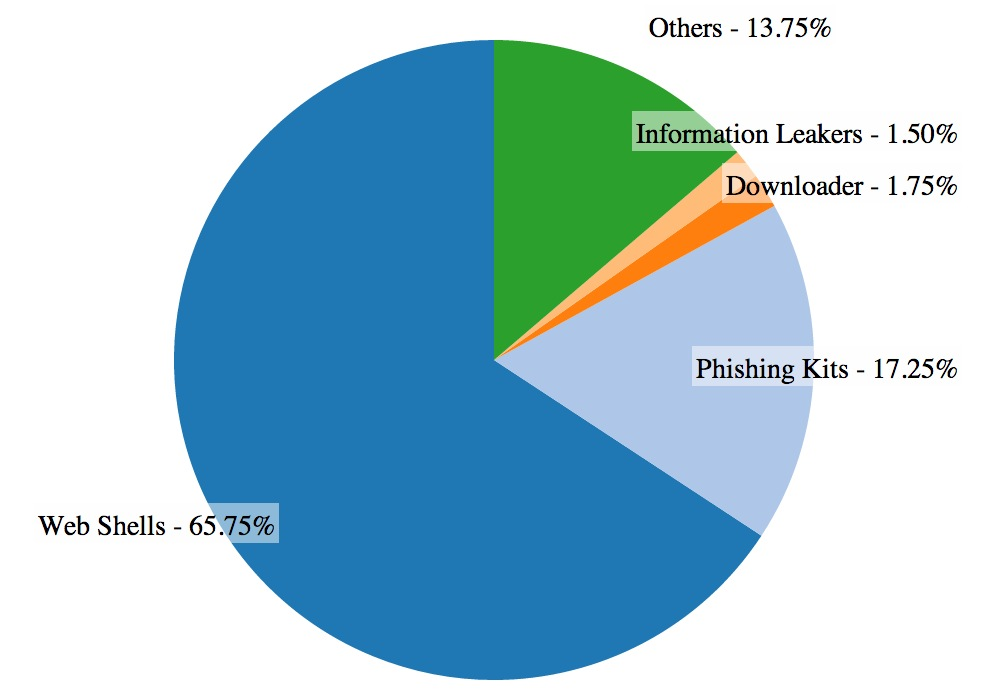
\includegraphics[width=0.7\textwidth]{Images/1stStageAttack.jpg}}
\caption{1st Stage attack file categorization.\label{fig:1stStageAttack}}
\end{figure}

The most remarkable side effect of every exploitation session is the upload or modification of files on the victim machine. Quite surprisingly, we noticed that when an exploitation session uploads a file, the file is uploaded in average 9.75 times. This strange behavior can be explained by the fact that most of the exploitation tools are automated, and since the attacker does not check in real-time whether each exploit succeeded or not, uploading the same file multiple times can increase the chance for the file to be successfully uploaded at least once. Results of this phase, resumed in Figure~\ref{fig:1stStageAttack}, show that the files uploaded during attack sessions consist, in 65.75\% of the cases, in web shells, in 17.25\% of the cases in phishing files (single HTML pages or complete phishing kits), in 1.75\% of the cases in scripts that automatically try to download and execute files from remote URLs, and in 1.5\% of the cases in scripts for local information gathering. The remaining 13.75\% of the files include malwares, defacement pages and several other categories.

\begin{figure}[tbh]
\centerline{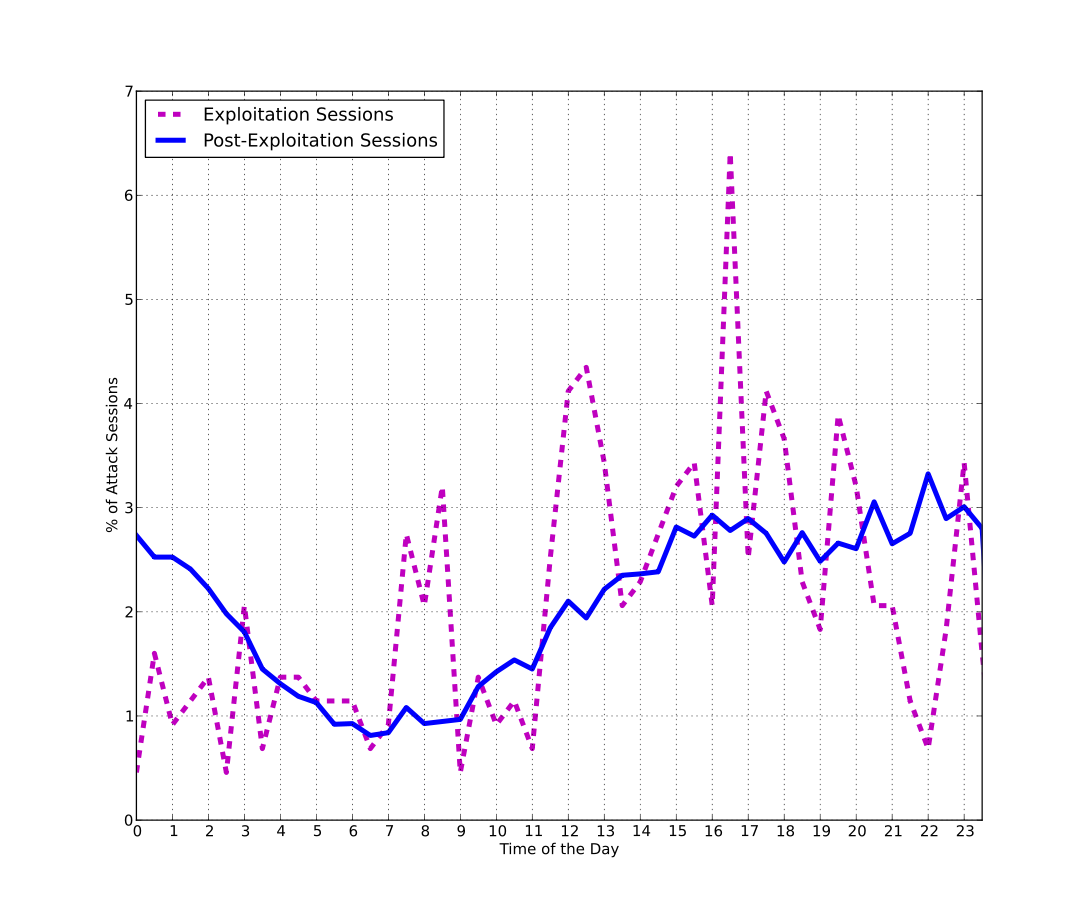
\includegraphics[width=0.7\textwidth]{Images/normalizedAttackTimes.png}}
\caption{Normalized time of attack sessions.\label{fig:normalizedAttackTimes}}
\end{figure}

Figure~\ref{fig:normalizedAttackTimes} shows the normalized times of the attacks received by our honeypots. The values were computed by adjusting the actual time of the attack with the timezone extracted from the IP geolocalization. It must be noticed that, using this method, we can have some false values in case the attacker is proxying its connection through an IP in a different part of the world. However, the graph shows a clear daylight trend for both the exploitation and post-exploitation phases. In particular, for the interactive sessions we observed fewer attacks performed between 4am and 10am, when probably also the criminals need to get some sleep. Interestingly, also the exploitation phase, that is mostly automated, shows a similar trend (even though not as clear). This could be the consequence of scans performed by botnet infected machines, some of which are probably turned off by their users during the night.

\subsubsection{Forum Activity}

Since the 1st day of operation, our forum application received a very large amount of traffic. Most of it came from automated spamming bots that kept flooding the forum with fake registrations and spam messages. We analyzed every snapshot of the machine's database in order to extract information about the forum's posts and the URLs that were embedded in each of them. This allowed us to identify and categorize several spam and link farming campaigns, as well as finding some rogue practices such as selling forum accounts.

A total of 68,201 unique messages were posted on the forum during our study, by 15,753 users using 3,144 unique IP addresses. Daily statistics on the forum show trends that are typical of medium to high traffic message boards: an average of 604 posts per day (with a max of 3085), with an average of 232 online users during peak hours (max 403).
Even more surprising than the number of posts is the number of new users registered to the forum: 1907 per day in average, and reaching a peak of 14,400 on October 23, 2013. We measured that 33.8\% of the IP addresses that performed actions on our forum were responsible of creating at least one fake account, but never posted any message. This finding suggests there are some incentives for criminals to perform automatic user registrations, and perhaps selling user accounts is even more profitable than the spamming activity itself. Our hypothesis is that, in some cases, forum accounts can be sold in bulk to other actors in the black market. We indeed found 1,260 fake accounts that were created from an IP address and then used few days later by other, different IPs, to post messages. This does not necessarily validate our hypothesis, but shows at least that forum spamming has become a complex ecosystem and it is difficult, nowadays, to find only a single actor behind a spam or link farming campaign.

\begin{figure}[tbh]
\centerline{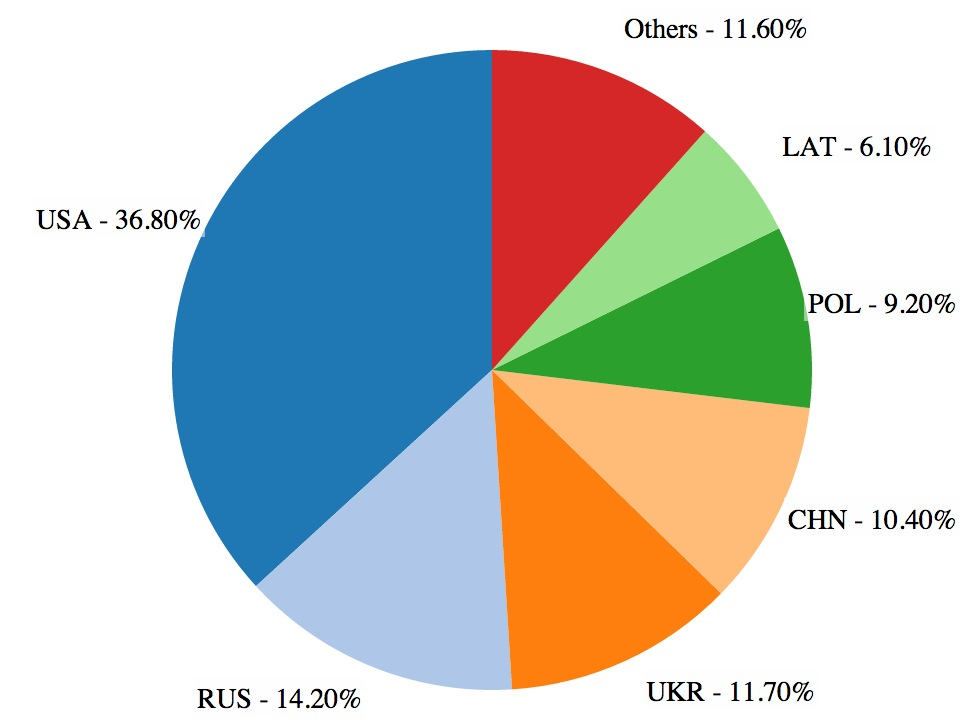
\includegraphics[width=0.7\textwidth]{Images/spamCountriesIP.jpg}}
\caption{Country provenance of IPs active on forum (message posting or registration).\label{fig:spamCountriesIP}}
\end{figure}

We tracked the geolocation of IP addresses responsible for registering users and posting to the forum. We identified the countries which are the most active on this category of rouge activity as the United States and Eastern Europe countries (mostly Russia, Ukraine, Poland, Latvia, Romania), as shown in Figure~\ref{fig:spamCountriesIP}. A total of 6687 distinct IP addresses were active on our forum (that is, posted at least one message or registered one or more accounts). Among these, 36.8\% were associated to locations in the US, while 51.6\% came from one of the cited Eastern European countries. The country coverage drastically changes if we consider only IP addresses that posted at least one message to the forum (ref Figure~\ref{fig:spamCountriesMessage}). In this case, IPs from the United States represent, alone, 62.3\% of all the IP addresses responsible for posting messages (Eastern Europe IPs in this case represent 21.2\% of the total), while we have much more variety in the number of different countries involved in the activity. This behavior strongly suggests a country-related specialization in malicious activities, where a small number of attackers in few areas sell on the black market the results of their activities to foreign agents, who perform different activities.

\begin{figure}[tbh]
\centerline{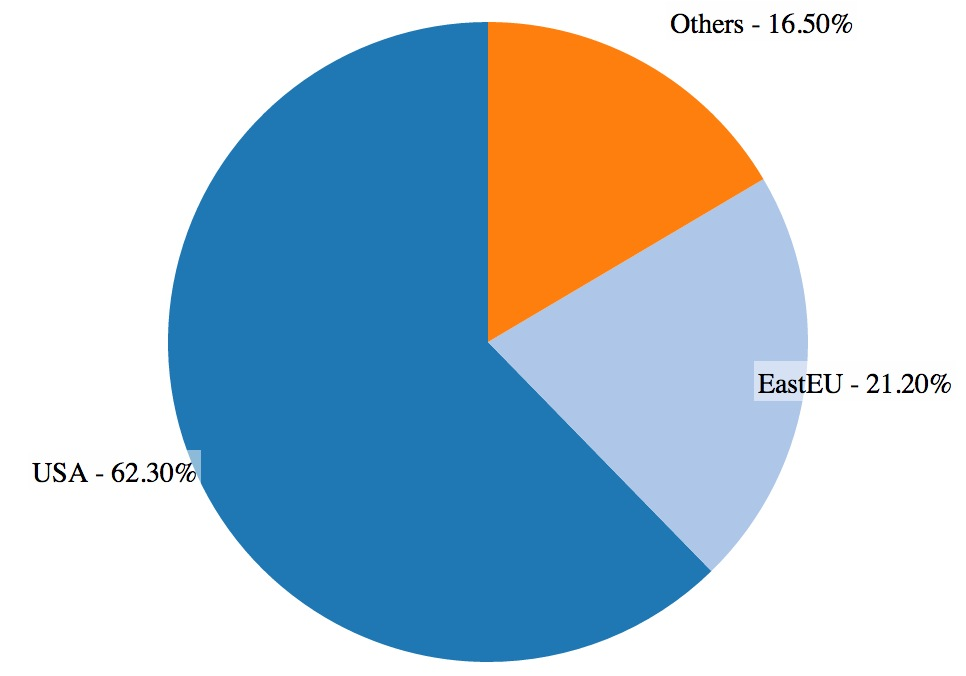
\includegraphics[width=0.7\textwidth]{Images/spamCountriesMessage.jpg}}
\caption{Country provenance of IPs posting at least one message.\label{fig:spamCountriesMessage}}
\end{figure}

Finally, we performed a simple categorization on all the messages posted on the forum, based on the presence of certain keywords. This allowed us to quickly identify common spam topics and campaigns. Thanks to this method, we were able to automatically categorize 63,763 messages (93.5\% of the total).
As shown in Figure~\ref{fig:SpamCategory}, the trends we extracted from message topics reveal that the most common category is drugs (45.2\% of the categorized messages, and showing peaks of 2000 messages per day), followed by search engine optimization (SEO, 17.4\%), electronics (13.5\%), adult content (7.9\%), and health care(5.2\%).
All the links inserted in the forum posts underwent an in-depth analysis using two automated, state-of-the-art tools for the detection of malicious web pages, namely Google Safe Browsing \cite{googleSafeBrowsing} and Wepawet \cite{wepaWet}. The detection results of these two tools show that, on the 221,423 URLs we extracted from the forum posts, a small but not insignificant fraction (2248, roughly 1 out of 100) consisted in malicious or possibly harmful links.

\begin{figure}[tbh]
\centerline{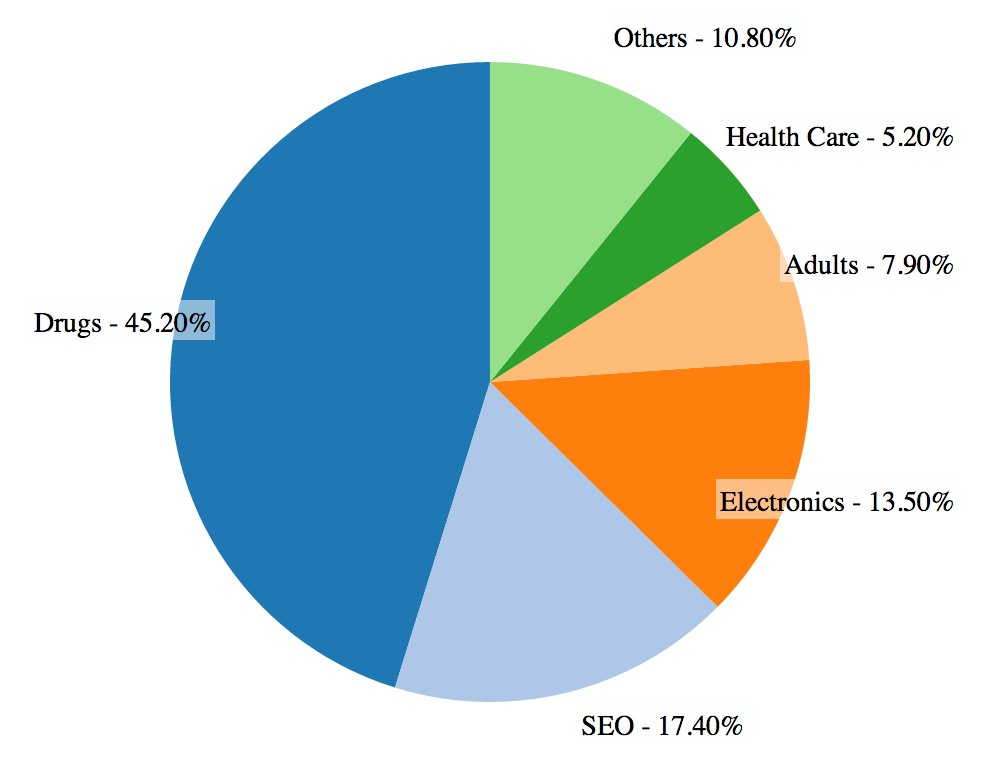
\includegraphics[width=0.7\textwidth]{Images/SpamCategory.jpg}}
\caption{Categories of spam messages.\label{fig:SpamCategory}}
\end{figure}

\subsection{Post-Exploitation}

The post-exploitation phase includes the analysis of the interaction between the attackers and the compromised machines. In our case, this is mostly done through the web shells installed during the exploitation phase or through the access to the public shells that we already pre-installed in our virtual machines.

The analysis of the post-exploitation phase deserves special attention since it is made of interactive sessions in which the attackers can issue arbitrary commands. However, these web shells do not have any notion of session: they just receive commands via HTTP requests and provide the responses in a state-less fashion. We decided to identify an ``interactive sessions'' every time a sequence of more than 3 commands is issued from the same IP and the idle time between consecutive commands is less than 5 minutes.
Over a total of 74,497 shell commands received, we registered 232 interactive sessions with an uploaded webshell and 8268 with one of our pre-installed shells. Because of the minimum number of commands threshold we imposed for the identification of a session only 52,368 shell commands have been included in a session. The majority of the commands not included in a session are single file uploads through one of our pre-installed webshells, mostly for defacement purposes.

The average session duration was of 5 minutes and 37 seconds, however, we registered 9 sessions lasting more than one hour each. The longest, in terms of commands issued to the system, was from a user in Saudi Arabia that sent 663 commands to the shell, including the manual editing of several files. Interestingly, one of the most common actions performed by users during an attack is the upload of a custom shell, even if the attacker broke into the system using a shell that was already available on the website. The reason for this behavior is that attackers know that, with a high probability, shells already installed on a system will contain backdoors and most likely leak information to their owner. In addition to the 17 web shells supported by our tools, we also identified the HTTP patterns associated to the most common custom shells uploaded by the attackers, so that we could parse the majority of commands issued to them.
In 83\% of the cases, attackers tried to use at least one active command (uploading or editing a file, changing file permissions, creating files or directories, scanning hosts, killing a process, connecting to a database, sending emails, etc.). The remaining sessions were purely passive, with the attackers only browsing our system and downloading source and configuration files.
Finally, in 61\% of the sessions the attackers uploaded a new file, and in 50\% of them they tried to modify a file already on the machine (in 13\% of the cases to perform a defacement). Regarding individual commands, the most commonly executed were the ones related to listing and reading files and directories, followed by editing files, uploading files, running commands on the system, listing the processes running on the system, and downloading files.

During this phase most of the attackers created or uploaded a new file: as can be seen in Figure~\ref{fig:2ndStageAttack}, there is much more variety in the category of files uploaded, as during this stage the attackers is trying to accomplish a certain goal rather than just obtain an access to the machine. The results do not consider attacks where a webshell is uploaded, as we still consider this action to be a 1st stage attack.

\begin{figure}[tbh]
\centerline{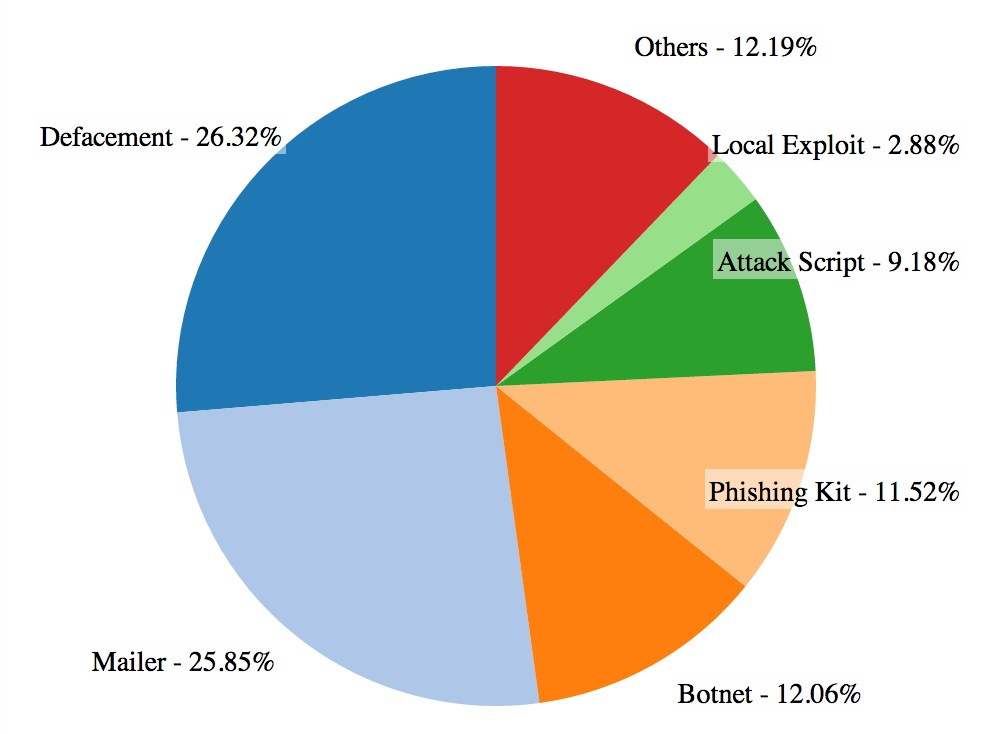
\includegraphics[width=0.7\textwidth]{Images/2ndStageAttack.jpg}}
\caption{2nd Stage Attack File Categorization\label{fig:2ndStageAttack}}
\end{figure}

It's evident how the variety of files is increased. In the next chapter we are going to explore in details attackers goals and single file categories, we provide here a first introduction to the various categories:

\begin{description}
\item[Defacement] The most common type of file uploaded, it's usually just an HTML document with the name of the attacker/team who performed the malicious activity;
\item[Mailer] A mailer is a script (usually written in PHP or Perl) for spamming purposes, it usually tries to read a list of e-mail addresses and sends the same message to each of them;
\item[Botnet] these scripts communicate with other machines for performing several tasks, transforming the hosting machine in a bot which receives and execute commands sent by others;
\item[Phishing Kit] it's a collection of HTML pages, images and CSS files, usually uploaded as compressed archives, looking like a ``famous'' website in order to fool a victim to insert their credentials. The most common copied website is Paypal, followed by Visa and FaceBook;
\item[Attack Scripts] This is a general category for including every script that is able to look for other websites and automatically exploit them. They usually accept a list of urls and, for each of them, they try to exploit a known vulnerability (like a vulnerable plugin for Joomla, etc);
\item[Local Exploits] This category relies with files that are trying to compromize the same machine they are running on, usualdly by means of privilege escalation.
\end{description}

Other categories include Uploaders, SQL dumpers, Malwares, Network Scanners, Drive-by Downloads, Flooder Scripts etc.

\section{Attackers Goals}

In this section we shift the focus from the way the attacks are performed to the motivation behind them. In other words, we try to understand what criminals do after they compromise a web application, and why. We discovered several goals attackers try to achieve after exploiting a machine: some of them are just looking for public recognition, some others are trying to create a botnet for profit, others are involved in spamming and phishing campaigns.

\begin{table}[tbh] % per piazzare la tabella t:top b:bottom h:here in ordine di preferenza; h è sconsigliato
\begin{center}
\begin{tabularx}{\textwidth}{|c|X|X|}
\hline
\textit{Category} & \textit{Unique Files} & \textit{Total Number Of Files} \\
\hline
Fake Downloads & 24 & 24 \\
Code Inclusion & 177 & 242 \\
Malicious Files Discovery & 216 & 217 \\
Java Applet & 221 & 225 \\
Drive-by Download & 284 & 310 \\
SQL dumper & 287 & 292 \\
Proxy & 335 & 343 \\
System Info Leaker & 341 & 387 \\
Mass Defacer & 356 & 383 \\
WebSearch Bot & 413 & 425 \\
Network Scanner & 420 & 445 \\
Malware & 475 & 492 \\
Documents & 516 & 518 \\
Uploader & 597 & 740 \\
Configuration Overloader & 656 & 713 \\
Backdoor & 703 & 728 \\
Bruteforcer Script & 2457 & 2659 \\
Local Exploit & 3033 & 3322 \\
Flooder Script & 3341 & 3452 \\
Attack Script (to other machines) & 4956 & 6064 \\
Botnet & 7878 & 8912 \\
Phishing Pack & 9445 & 18608 \\
Mailer & 13012 & 15324 \\
Defacement & 14698 & 18023 \\
Webshell & 20322 & 28551 \\
\hline \hline
Total & 85163 & 111399 \\
\hline
\end{tabularx}
\caption{Summary of files Received.\label{tab:webapps}}
\end{center}
\end{table}

We analyzed the files uploaded during the exploitation phase, and the ones created or modified during the post-exploitation phase. We normalized each file content, and we clustered them together according to their similarity, obtaining several clusters according to their ``purpose''. We identified a total of 25 categories, and the results are displayed in table~\ref{tab:webapps}. From the table we removed all broken files. The corresponding graphs shows the distribution of files according to their percentage.

\begin{figure}
\centering
\begin{subfigure}{.5\textwidth}
  \centering
  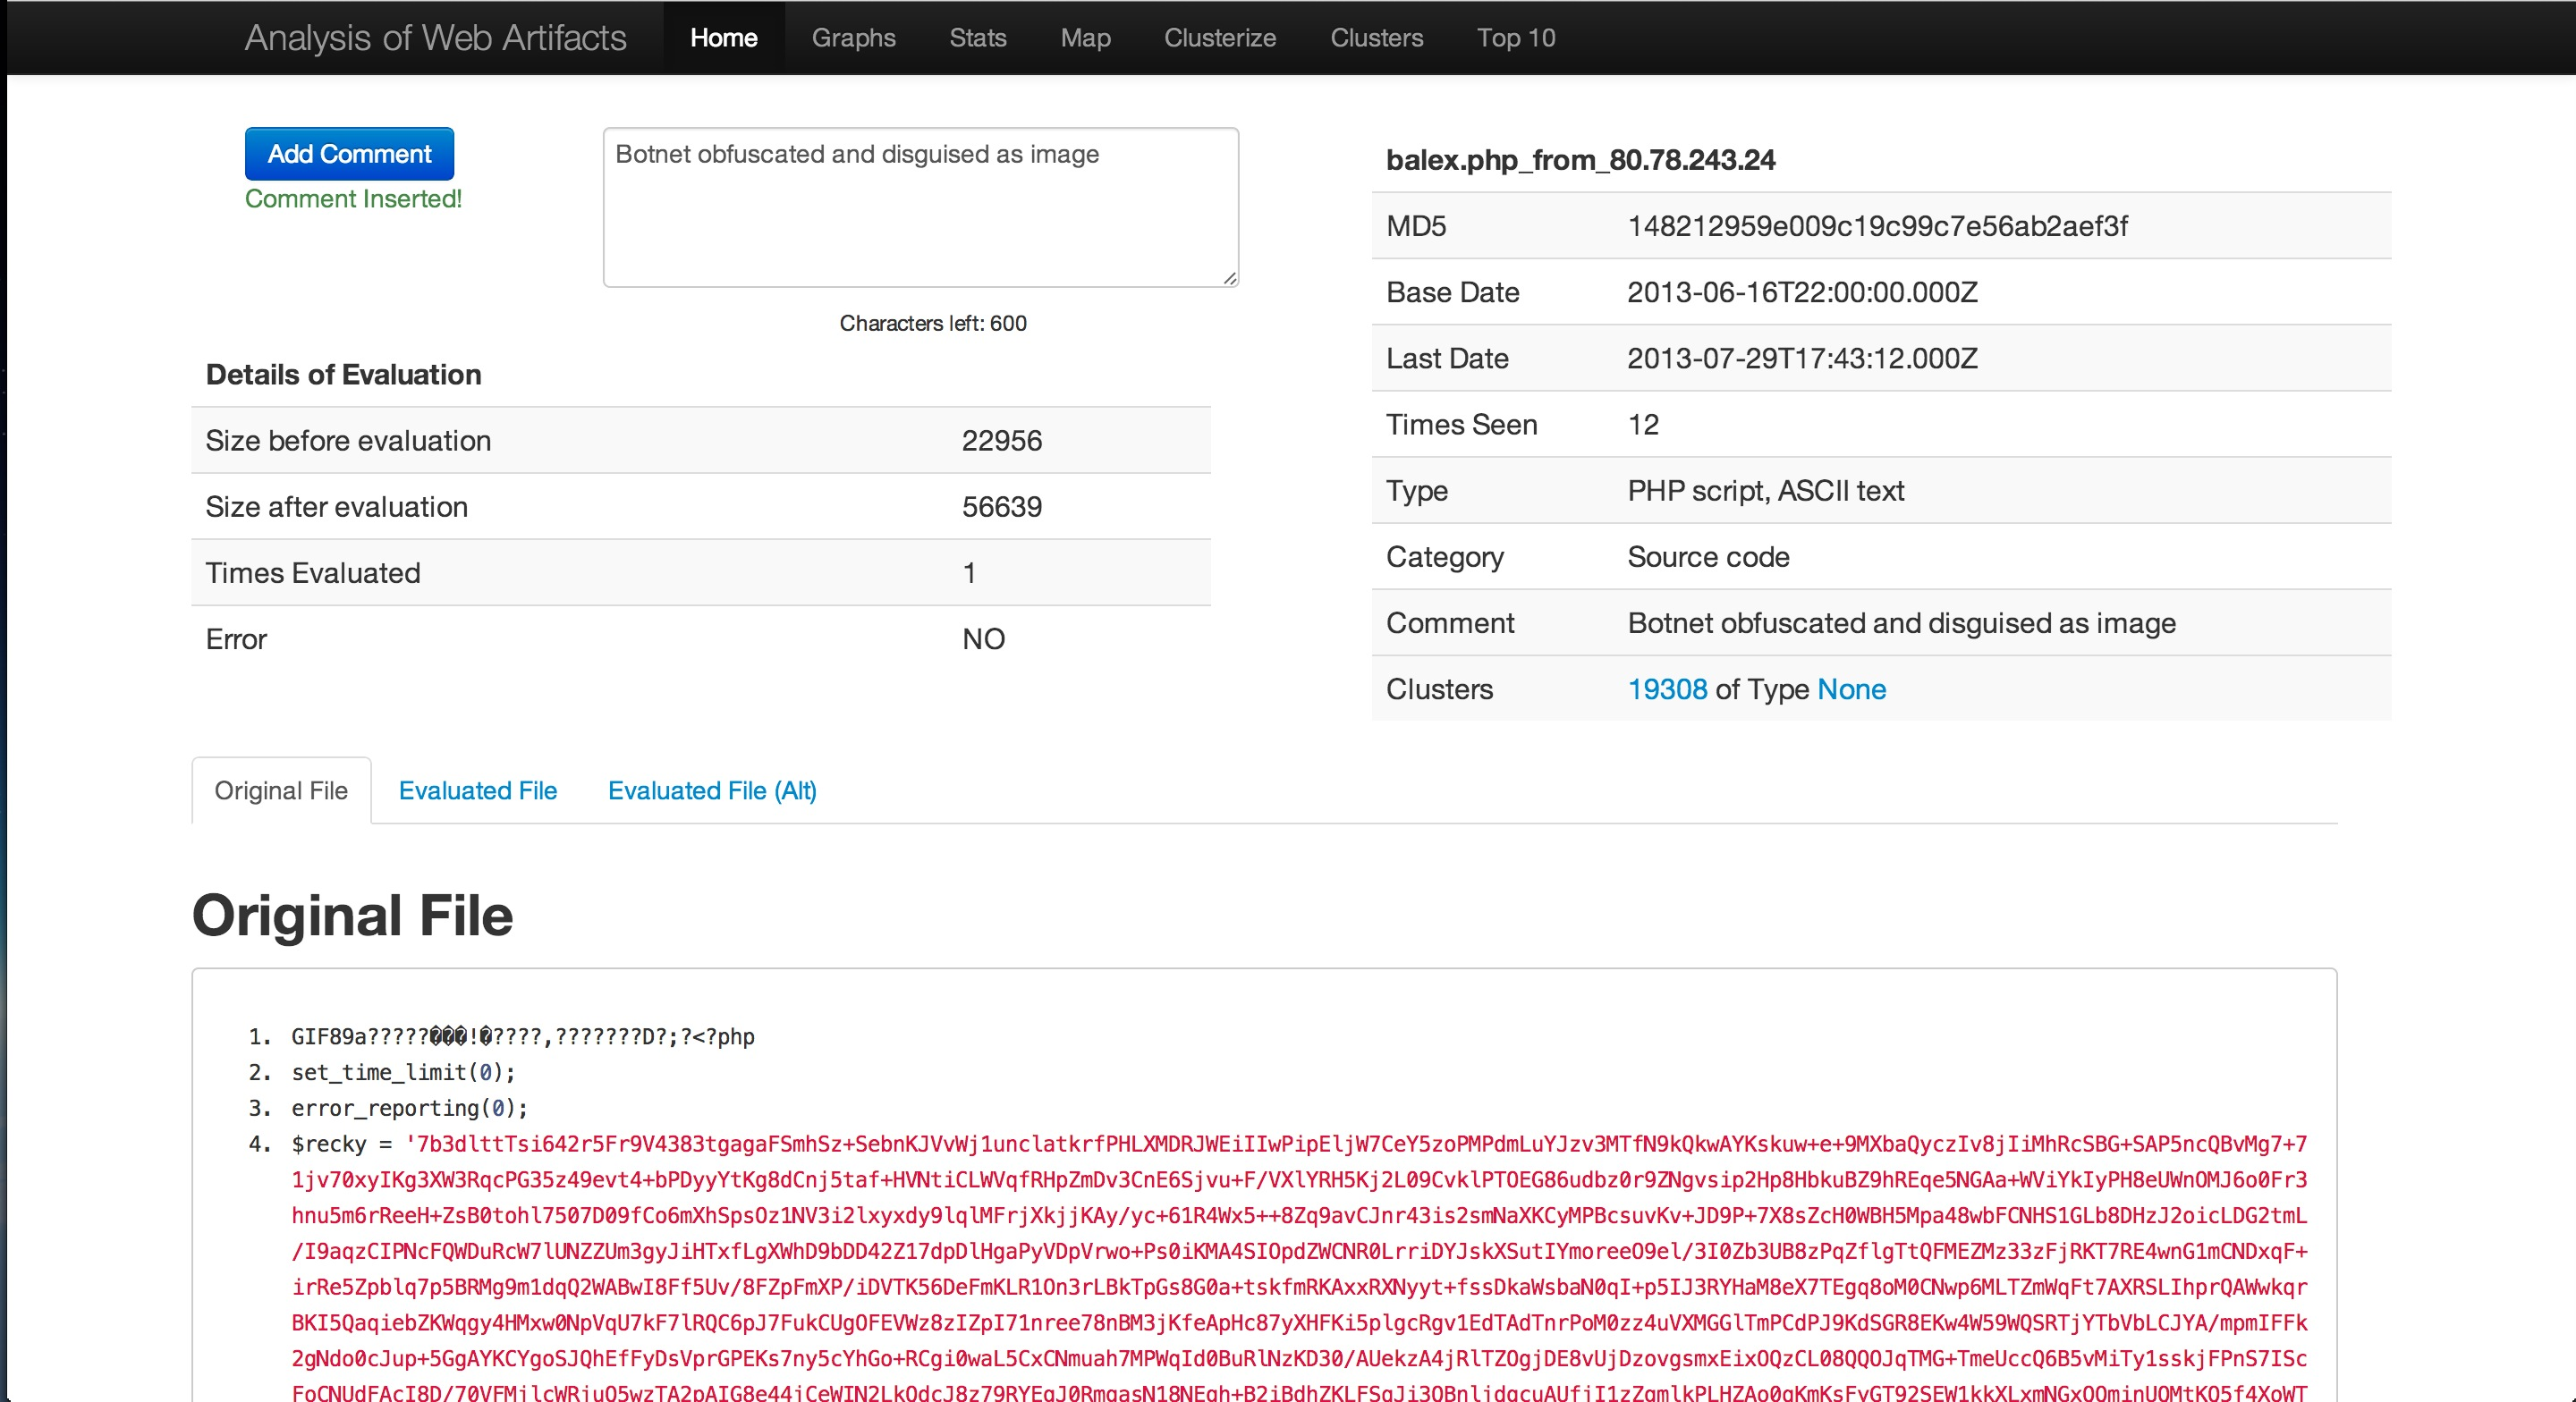
\includegraphics[width=1.0\linewidth]{Images/obf_file.jpg}
  \caption{Unique Files Distribution}
  \label{fig:sub1}
\end{subfigure}%
\begin{subfigure}{.5\textwidth}
  \centering
  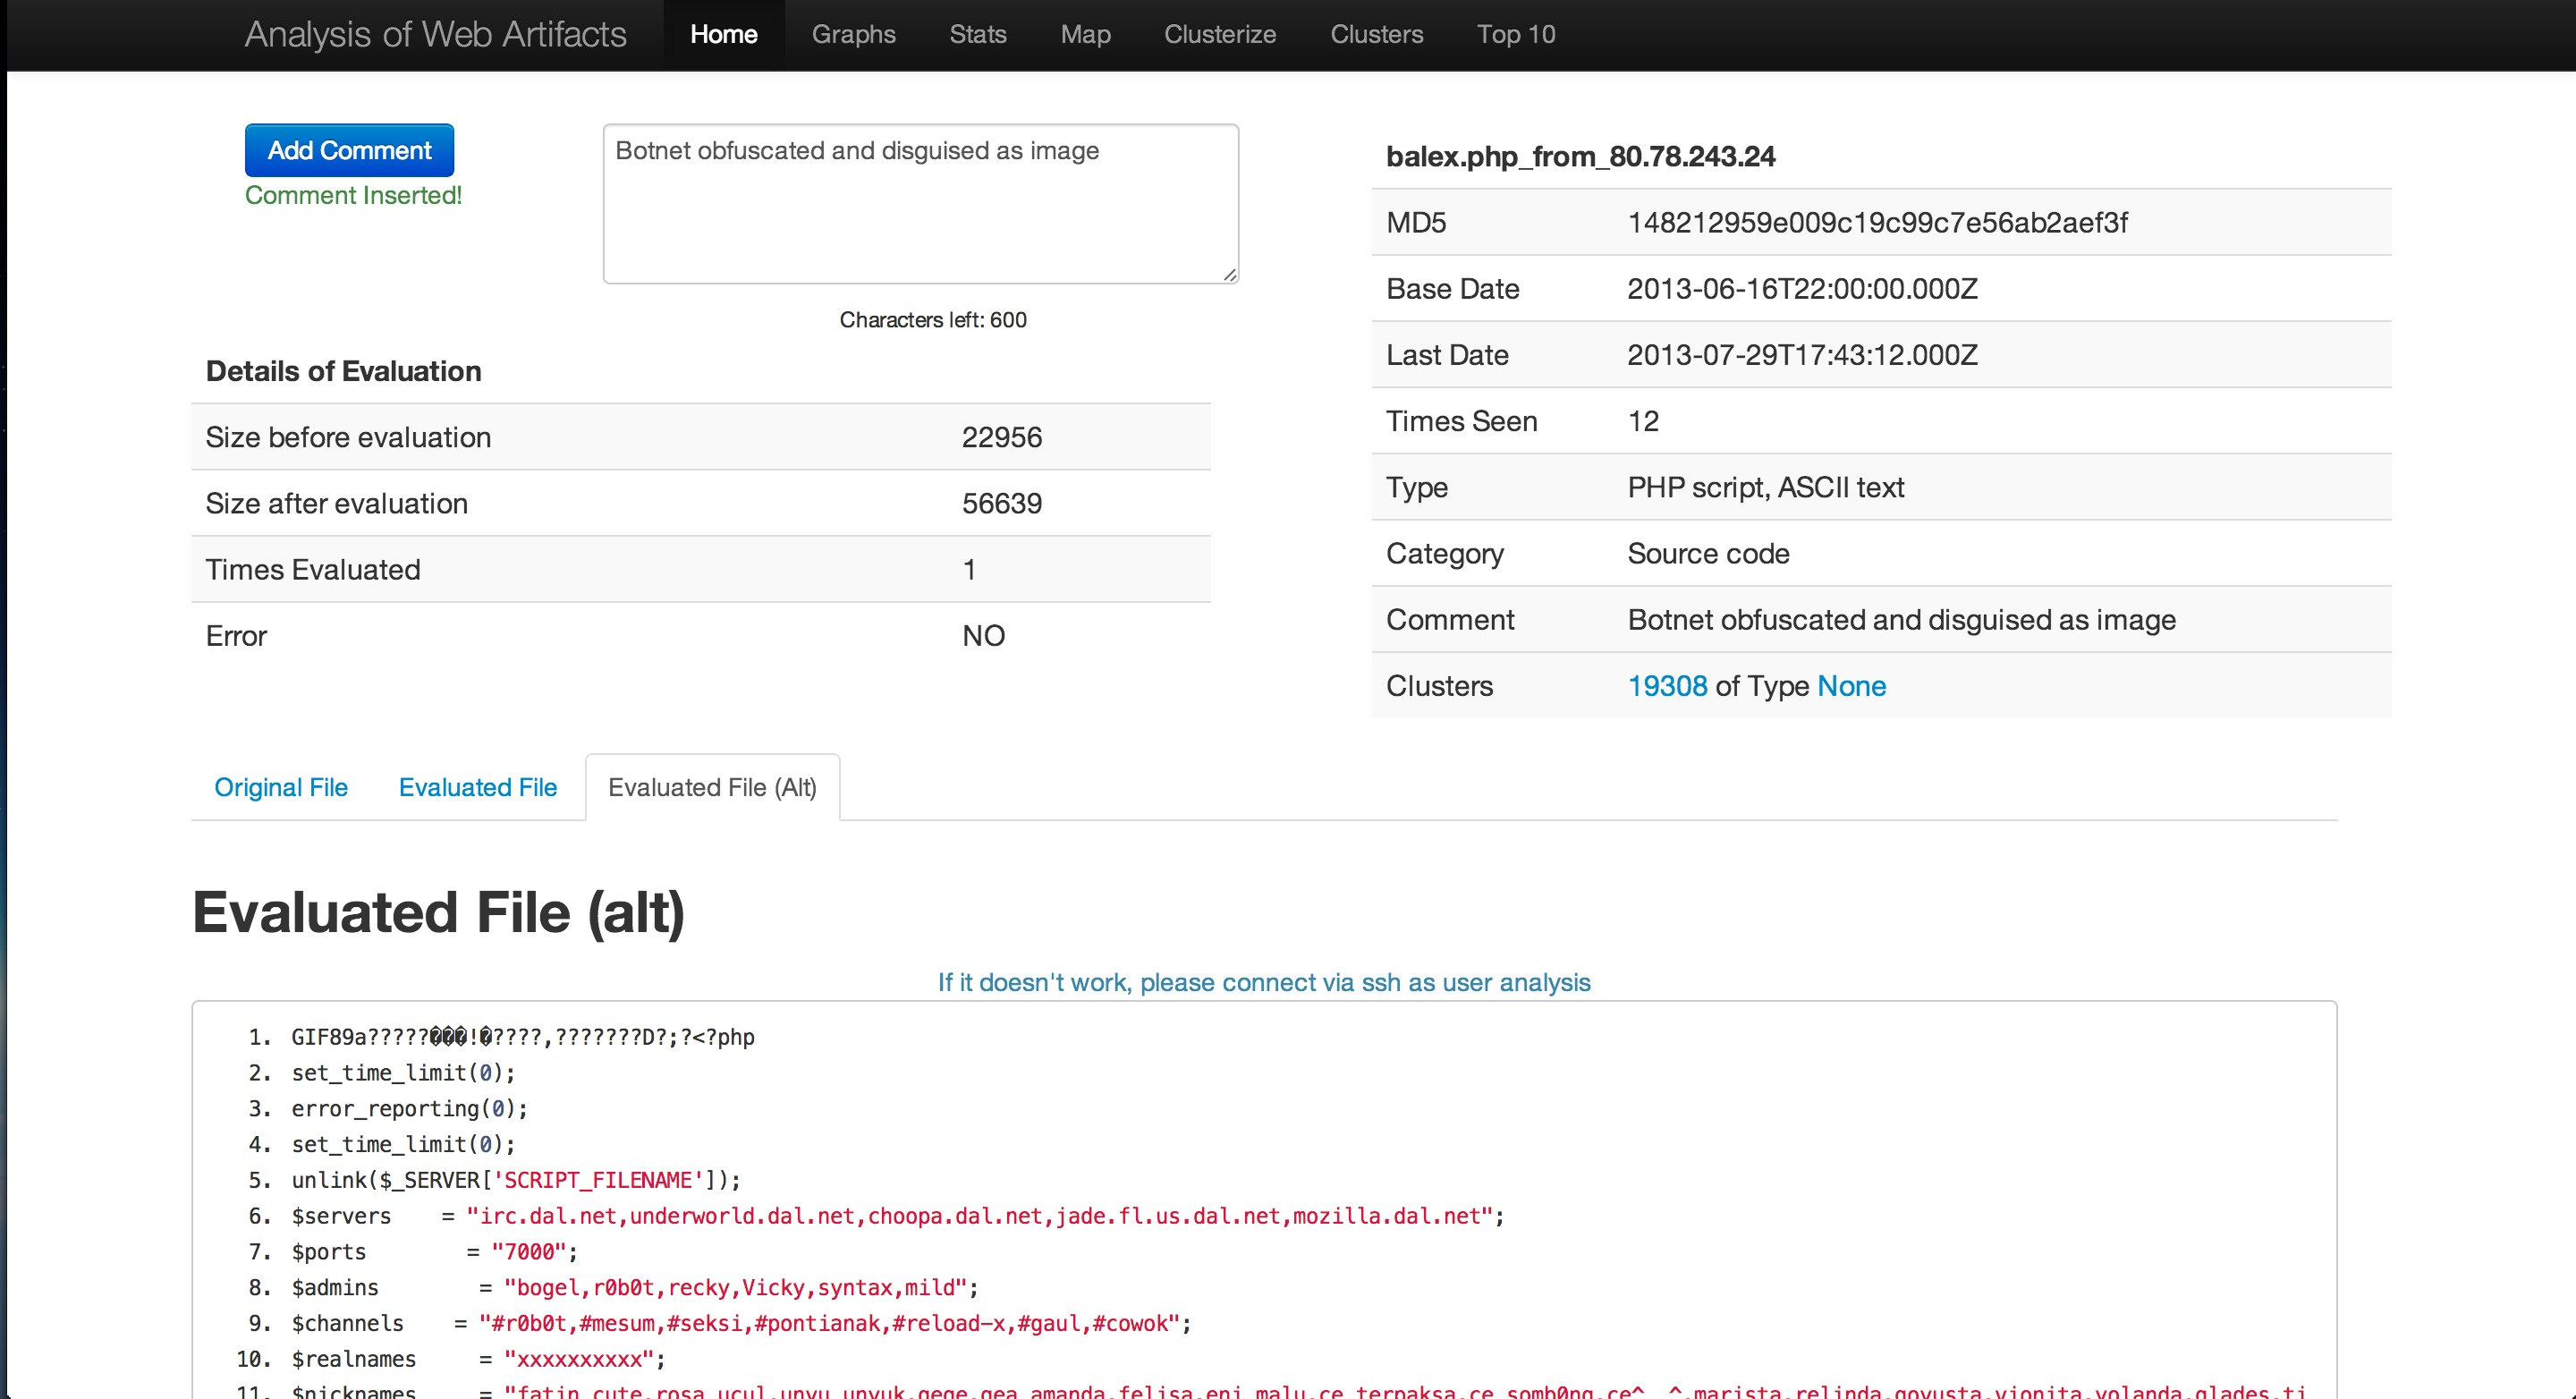
\includegraphics[width=1.0\linewidth]{Images/deobf_file.jpg}
  \caption{Total Files Distribution}
  \label{fig:sub2}
\end{subfigure}
\caption{Categorization of files received}
\label{fig:test}
\end{figure}

For example, 1.7\% of the unique files we observed in our experiments were used to try to escalate the privileges on the compromised machine. This is different from saying that 1.7\% of the attackers tried to escalate the privileges of the machine. Unfortunately, linking the files to the attacks in which they were used is not always possible. Therefore, we computed an estimation of the attackers that performed a certain action by identifying each unique IP that uploaded a certain file during an


\chapter{Conclusioni}

Qui si inseriscono brevi conclusioni sul lavoro svolto, senza ripetere inutilmente il sommario.

Si possono evidenziare i punti di forza e quelli di debolezza, nonché i possibili sviluppi futuri o attività da svolgere per migliorare i risultati.


% La bibliografia, da inserirsi solo se ci sono state citazioni.
% In questo caso ricordarsi che bisogna sempre elaborare due volte il file .TEX
% perché la prima volta viene generata la bibliografia mentre la seconda volta viene inclusa

% NOTA: citare il DOI non è obbligatorio ma MOLTO desiderabile

%\begin{thebibliography}{9} % se ci sono meno di 10 citazioni
\begin{thebibliography}{99} % se ci sono da 10 a 99 citazioni

\bibitem{stopbadawareSurvey}
Stop BadAware Survey for Compromised Websites
\url{http://www.stopbadware.org/files/compromised-websites-an-owners-perspective.pdf}

\bibitem{honeynetProject}
The Honeynet project, % nome del progetto
\url{http://www.honeynet.org/} % URI della pagina web

\bibitem{leurre}
F.Pouget, M.Dacier, V.H.Pham
``Leurre.com: on the advantages of deploying a large scale distributed honeypot platform''
ECCE 2005, E-Crime and Computer Conference, March 29-30 2005,
Monaco, France
pp.\ 29-30

\bibitem{sgnet}
C.Leita, M.Dacier,
``Sgnet: A worldwide deployable framework to support the analysis of malware threat models''
EDCC 2008, 7th European Dependable Computing Conference,
Kaunas, Lituania, May 7-9, 2008
\doi{10.1109/EDCC-7.2008.15}

\bibitem{honeyd}
N. Provos,
``A virtual honeypot framework'',
USENIX Security Symposium,
San Diego (California - USA), August 9-13, 2004,
pp.\ 1-14

\bibitem{highhoney}
V. Nicomette, M. Kaaniche, E. Alata, and M. Herrb,
``Set-up and Deployment of a High Interaction Honeypot: Experiment and Lessons Learned'',
Journal in Computer Virology,
vol.\ 7, no.\ 2,
May 2011,
pp.\ 143-157,
\doi{10.1007/s11416-010-0144-2}

\bibitem{googleHoney}
Google Hack Honeypot,
\url{http://ghh.sourceforge.net}

\bibitem{dswhp}
DShield web honeypot project,
\url{https://sites.google.com/site/webhoneypotsite/}

\bibitem{spitzhoney}
To Build A Honeypot, Lance Spitzner,
\url{http://www.spitzner.net/honeypot.html}

\bibitem{glastopf}
Glastopf project,
\url{http://honeynet.org/files/KYT-Glastopf-Final_v1.pdf}

\bibitem{johnhsh}
J. P. John, F. Yu, Y. Xie, A. Krishnamurthy, M. Abadi,
``Heat-seeking honeypots: design and experience'',
International World Wide Web Conference (WWW),
New York (NY - USA), March-April 2011,
pp.\ 207-216,
\doi{10.1145/1963405.1963437}

\bibitem{hihat}
M. Muüter, F. Freiling, T. Holz, and J. Matthews,
``A generic toolkit for converting web applications into high-interaction honeypots''
Recent Advances in Intrusion Detection (RAID),
pp.\ 154-170,
Gold Coast (Australia), September 5-7, 2007.

\bibitem{sshprofiling}
D.Ramsbrock, R.Berthier, and M.Cukier,
``Profiling attacker behaviour following ssh compromises''
IEEE/IFIP International Conference on Dependable Systems and Networks, 2007.
\doi{10.1109/DSN.2007.76}

\bibitem{plagdet1}
X. Chen, B. Francia, M. Li, B. Mckinnon, and A. Seker,
``Shared information and program plagiarism detection''
IEEE Transactions on Information Theory,
Vol.\ 50, No.\ 7,
July 2004,
pp.\ 1545-1551,
\doi{10.1109/TIT.2004.830793}

\bibitem{plagdet2}
A. Saebjornsen, J. Willcock, T. Panas, D. Quinlan, and Z. Su,
``Detecting code clones in binary executables'',
International Symposium on Software testing and analysis, ISSTA 2009,
 Chicago (Illinois - USA), July 19-23, 2009,
pp.\ 117-128,
\doi{10.1145/1572272.1572287}

\bibitem{ssdeep}
J. Kornblum,
``Identifying almost identical files using context triggered piecewise hashing'',
Digital Investigation,
Vol. 3, Supplement(0)
2006.
pp.\ 91-97,
\doi{:10.1016/j.diin.2006.06.015}

\bibitem{sdhash}
V. Roussev,
``Data fingerprinting with similarity digests''
Advances in Digital Forensics VI, volume 337,
Springer Boston, 2010,
pp.\ 207-226,
\doi{10.1007/978-3-642-15506-2_15}

\bibitem{vmescape}
VMWare escape, % nome del progetto
\url{http://www.coresecurity.com/content/advisory-vmware} % URI della pagina web

\bibitem{phpMyAdmin}
phpMyAdmin reference page,
\url{http://www.phpmyadmin.net}

\bibitem{osCommerce}
osCommerce reference page,
\url{http://www.oscommerce.com}

\bibitem{joomla}
Joomla! reference page,
\url{http://www.joomla.org}

\bibitem{wordpress}
Wordpress reference page,
\url{http://www.wordpress.com}

\bibitem{smf}
SMF reference page,
\url{http://www.simplemachines.org}

\bibitem{drupal}
Drupal reference page,
\url{http://www.drupal.org}

\bibitem{conntrack}
Conntrack reference page
\url{http://www.netfilter.org/projects/libnetfilter_conntrack/index.html}

\bibitem{libmagic}
LibMagic Debian package page
\url{http://packages.debian.org/unstable/libdevel/libmagic-dev}

\bibitem{phpcrypt}
php-crypt home page
\url{http://www.php-crypt.com}

\bibitem{webdeobf}
PHP deobfuscation web service
\url{https://www.whitefirdesign.com/tools/deobfuscate-php-hack-code.html}

\bibitem{evalhook}
EvalHook PHP extension, by Stefan Esser
\url{http://php-security.org/2010/05/13/article-decoding-a-user-space-encoded-php-script}

\bibitem{spamsum}
SpamSum spam detection system, first example of context-triggered hash
\url{https://www.samba.org/ftp/unpacked/junkcode/spamsum/}

\bibitem{md5}
MD5 RFC 1321
\url{http://www.ietf.org/rfc/rfc1321.txt}

\bibitem{node_home}
Node.Js homepage
\url{http://nodejs.org/}

\bibitem{express_node}
Express framework homepage
\url{http://expressjs.com/}

\bibitem{d3_home}
d3 homepage
\url{http://d3js.org/}

\bibitem{bootstrap}
Bootstrap homepage
\url{http://getbootstrap.com/2.3.2/}

\bibitem{devilfinder}
Devilfinder.com, search engine
\url{http://devilfinder.com}

\bibitem{googleSafeBrowsing}
Google Safe Browsing website
\url{http://www.google.com/transparencyreport/safebrowsing/}

\bibitem{wepaWet}
Wepawet home page
\url{https://wepawet.iseclab.org/}

\bibitem{jdgui}
JD-GUI home page
\url{http://jd.benow.ca/}

\bibitem{cveJava}
CVE-2013-0422 <Java7.11 RCE outside SandBox
\url{http://cvedetails.com/cve/2013-0422}

\bibitem{CVE-2010-0188}
CVE-2010-0188 Adobe Acrobat <8.21 and <9.21 RCE
\url{http://cvedetails.com/cve/2010-0188}

\bibitem{CVE-2010-1885}
CVE 2010-1885 MS Win XP Help Center URL Validation RCE
\url{http://cvedetails.com/cve/2010-1885}

\bibitem{nessus}
Nessus network scanner
\url{http://www.tenable.com/products/nessus}

\bibitem{nmap}
Nmap port mapper
\url{http://nmap.org/}

\bibitem{malwWin}
G-Data report For Malware OS percentages
\url{http://www.gdatasoftware.co.uk/press-center/news/article/article/1760-number-of-new-computer-viruses.html}

\bibitem{virustotal}
VirusTotal Home Page
\url{https://www.virustotal.com/}

\bibitem{joomlaImgManager}
Joomla! img\_manager Arbitrary File Upload vulnerability
\url{http://www.exploit-db.com/exploits/17734/}

\bibitem{irc}
IRC RFC 1459
\url{http://tools.ietf.org/html/rfc1459.html}

\bibitem{zoneh}
Zone-h home page
\url{https://www.zone-h.org/}

\bibitem{python}
Python home page
\url{https://www.python.org/}

\bibitem{perl}
Perl home page
\url{https://www.perl.org/}

\bibitem{php}
PHP home page
\url{https://www.php.net/}

\bibitem{curl}
cURL home page
\url{https://www.curl.haxx.se/}

\bibitem{apache}
Apache home page
\url{https://www.apache.org/}

\bibitem{mysql}
MySQL home page
\url{https://www.mysql.com/}

\bibitem{echolot}
Echolot home page
\url{http://www.palfrader.org/code/echolot/}

\end{thebibliography}



\end{document}
